%%% The main file. It contains definitions of basic parameters and includes all other parts.

%% Settings for single-side (simplex) printing
%\documentclass[12pt,a4paper]{report}
% \openright makes the following text appear on a right-hand page
%\let\openright=\clearpage

%% Settings for two-sided (duplex) printing
\documentclass[12pt,a4paper,twoside,openright]{report}

 \let\openright=\cleardoublepage

%% Generate PDF/A-2u
\usepackage[a-2u]{pdfx}

%% Character encoding: usually latin2, cp1250 or utf8:
\usepackage[utf8]{inputenc}

%% Prefer Latin Modern fonts
\usepackage{lmodern}

%% Further useful packages (included in most LaTeX distributions)
%\usepackage[backend=bibtex,style=alpha]{biblatex-trad}
\usepackage{amsmath}        % extensions for typesetting of math
\usepackage{amsfonts}       % math fonts
\usepackage{amsthm}         % theorems, definitions, etc.
\usepackage{bbding}         % various symbols (squares, asterisks, scissors, ...)
\usepackage{bm}             % boldface symbols (\bm)
\usepackage{graphicx}       % embedding of pictures
\usepackage{fancyvrb}       % improved verbatim environment
%\usepackage{natbib}         % citation style AUTHOR (YEAR), or AUTHOR [NUMBER]
%\usepackage[nottoc]{tocbibind} % makes sure that bibliography and the lists
			    % of figures/tables are included in the table
			    % of contents
\usepackage{dcolumn}        % improved alignment of table columns
\usepackage{booktabs}       % improved horizontal lines in tables
\usepackage{paralist}       % improved enumerate and itemize
\usepackage{xcolor}         % typesetting in color
\usepackage{siunitx}
\usepackage{todonotes}
\usepackage{cleveref}
\usepackage{subcaption}
\usepackage[linesnumbered,ruled,vlined]{algorithm2e}
%%% Basic information on the thesis



% Thesis title in English (exactly as in the formal assignment)
\def\ThesisTitle{Employing GPU to Process Data from Electron Microscope}

% Author of the thesis
\def\ThesisAuthor{Michal Bali}

% Year when the thesis is submitted
\def\YearSubmitted{2020}

% Name of the department or institute, where the work was officially assigned
% (according to the Organizational Structure of MFF UK in English,
% or a full name of a department outside MFF)
\def\Department{Department of Software Engineering}

% Is it a department (katedra), or an institute (ústav)?
\def\DeptType{Department}

% Thesis supervisor: name, surname and titles
\def\Supervisor{RNDr. Martin Kruliš, Ph.D}

% Supervisor's department (again according to Organizational structure of MFF)
\def\SupervisorsDepartment{Department of Software Engineering}

% Study programme and specialization
\def\StudyProgramme{Master of Computer Science}
\def\StudyBranch{Software Systems}

% An optional dedication: you can thank whomever you wish (your supervisor,
% consultant, a person who lent the software, etc.)
\def\Dedication{%
Dedication.
}

% Abstract (recommended length around 80-200 words; this is not a copy of your thesis assignment!)
\def\Abstract{%
Abstract.
}

% 3 to 5 keywords (recommended), each enclosed in curly braces
\def\Keywords{%
{GPU} {parallel} {data} {image} {pattern}
}

%% The hyperref package for clickable links in PDF and also for storing
%% metadata to PDF (including the table of contents).
%% Most settings are pre-set by the pdfx package.
\hypersetup{unicode}
\hypersetup{breaklinks=true}

% Definitions of macros (see description inside)
%%% This file contains definitions of various useful macros and environments %%%
%%% Please add more macros here instead of cluttering other files with them. %%%

%%% Minor tweaks of style

% These macros employ a little dirty trick to convince LaTeX to typeset
% chapter headings sanely, without lots of empty space above them.
% Feel free to ignore.
\makeatletter
\def\@makechapterhead#1{
  {\parindent \z@ \raggedright \normalfont
   \Huge\bfseries \thechapter. #1
   \par\nobreak
   \vskip 20\p@
}}
\def\@makeschapterhead#1{
  {\parindent \z@ \raggedright \normalfont
   \Huge\bfseries #1
   \par\nobreak
   \vskip 20\p@
}}
\makeatother

% This macro defines a chapter, which is not numbered, but is included
% in the table of contents.
\def\chapwithtoc#1{
\chapter*{#1}
\addcontentsline{toc}{chapter}{#1}
}

% Draw black "slugs" whenever a line overflows, so that we can spot it easily.
\overfullrule=1mm

%%% Macros for definitions, theorems, claims, examples, ... (requires amsthm package)

%\theoremstyle{plain}
%\newtheorem{thm}{Theorem}
%\newtheorem{lemma}[thm]{Lemma}
%\newtheorem{claim}[thm]{Claim}

%\theoremstyle{plain}
%\newtheorem{defn}{Definition}

%\theoremstyle{remark}
%\newtheorem*{cor}{Corollary}
%\newtheorem*{rem}{Remark}
%\newtheorem*{example}{Example}

%%% An environment for proofs

\newenvironment{myproof}{
  \par\medskip\noindent
  \textit{Proof}.
}{
\newline
\rightline{$\qedsymbol$}
}

%%% An environment for typesetting of program code and input/output
%%% of programs. (Requires the fancyvrb package -- fancy verbatim.)

\DefineVerbatimEnvironment{code}{Verbatim}{fontsize=\small, frame=single}

%%% The field of all real and natural numbers
\newcommand{\R}{\mathbb{R}}
\newcommand{\N}{\mathbb{N}}

%%% Useful operators for statistics and probability
%\DeclareMathOperator{\pr}{\textsf{P}}
%\DeclareMathOperator{\E}{\textsf{E}\,}
%\DeclareMathOperator{\var}{\textrm{var}}
%\DeclareMathOperator{\sd}{\textrm{sd}}

%%% Transposition of a vector/matrix
\newcommand{\T}[1]{#1^\top}

%%% Various math goodies
\newcommand{\goto}{\rightarrow}
\newcommand{\gotop}{\stackrel{P}{\longrightarrow}}
\newcommand{\maon}[1]{o(n^{#1})}
\newcommand{\abs}[1]{\left|{#1}\right|}
\newcommand{\dint}{\int_0^\tau\!\!\int_0^\tau}
\newcommand{\isqr}[1]{\frac{1}{\sqrt{#1}}}

%%% Various table goodies
\newcommand{\pulrad}[1]{\raisebox{1.5ex}[0pt]{#1}}
\newcommand{\mc}[1]{\multicolumn{1}{c}{#1}}

\newcommand{\norm}[1]{\left\lVert#1\right\rVert}

\DeclarePairedDelimiter\ceil{\lceil}{\rceil}
\DeclarePairedDelimiter\floor{\lfloor}{\rfloor}

\newcommand\IT[1]{\textit{#1}}

\newcommand\XX[1]{{\color{red} #1}}


% Title page and various mandatory informational pages
\begin{document}
\include{title}

%%% A page with automatically generated table of contents of the master thesis

\tableofcontents

%%% Each chapter is kept in a separate file
\chapter*{Introduction}
\addcontentsline{toc}{chapter}{Introduction}

Physics is constantly developing new methods how to describe and measure the reality around us. Nowadays, it is easily possible to collect vast amount of data, however it is useless unless we are able to analyze it efficiently. This thesis aims to help analysis of data used to study the microstructure of materials.

Electron backscatter diffraction (EBSD) is a scientific tool used to examine crystalline materials. It is based on an electron microscope shooting a beam of electrons towards the studied specimen. They are then reflected off the surface and captured by a camera, resulting in a grayscale image of the \emph{backscatter pattern}. Physicists then study the deformation of those patterns to determine several characteristics of the crystalline material such as crystal orientation, phase or elastic strain.

In 2006, Wilkinson, Meaden and Dingley first described the technique of high resolution EBSD analysis \cite{wilkinson2006high}. It is based on cross--correlating several subregions of a deformed and reference (undeformed) images. The cross-correlation is then processed to obtain shifts between the regions of interest with subpixel accuracy by interpolating between the points of best correlation match. From the shifts, it is possible to determine elastic strain and lattice rotation of the crystalline material.

When examining an object using EBSD, the procedure has to be repeated thousands or even millions of times. Usually, the images are taken in a raster that covers the area of interest which produces thousands of images. For each image, the analysis involves cross correlating tens of subregions ($100\times100$ pixels), which is computationally expensive. At the same time, processing of individual subregions is independent that makes it possible to leverage data parallelism and thus is appropriate for implementation on modern GPUs.

Faster processing of patterns enables the physicists to process bigger datasets that cover larger areas with higher resolution. Current commercially available software is insufficient for larger EBSD maps, which can contain up to million of patterns and the analysis takes tens of hours. A fast GPU implementation has the potential to drastically improve the situation.

Modern EBSD cameras are also able to take hundreds of images per second depending on image quality. That means it is possible to create large datasets in a reasonable amount of time and the analysis is the bottleneck of the process. Reference python implementation, that has been provided by physicists from Department of Physics of Material at Charles University in Prague, can process from 5 to 50 patterns per second, depending on the input parameters.

In this thesis we analyze the technique used to process the EBSD data from performance point of view, implement the most computationally expensive parts using the CUDA technology and benchmark the implementation.



\chapter{Processing of electron backscatter patterns}
\label{chap1}

Electron microscopes are used in many scientific fields to study microstructure of materials. They rely on electrons instead of photons, which allows them to achieve greater magnification than light microscopes. The microscope emits a beam of electrons, which interact with the specimen, either transmitting through it or reflecting back. The electrons therefore carry an information about the specimen. We capture them on a phosphor screen which emits light and then we take a picture of the screen by a camera, so the result of one electron microscope measurement is an image.

One measurement of electron microscope gets information about only one microscopic point in the specimen. However sometimes we need to map a larger area of the material. For this purpose, scientists use a \emph{scanning electron microscope}. It is a device that repeatedly emits an electron beam towards the specimen, scanning the surface in a raster pattern. So it does the measurement in one place, then moves a bit (e.g. $\SI{1}{\nano\meter}$ aside) and repeats. Since we are measuring the micro world, it takes thousands of iterations to scan a reasonably large area of the specimen. For example, test data that we used contained over 15000 images taken in a $120 \times 120$ raster covering an area of the specimen surface approximately $\SI{70}{\nano\meter} \times \SI{70}{\nano\meter}$ big.

We process data obtained using the \emph{electron backscatter diffraction} which is a scientific method that utilizes the scanning electron microscope to study crystalline materials (i.e., materials with a highly ordered microscopic structure). The principle of the electron backscatter diffraction is sketched in \cref{ebsd-principle}. When a beam of electrons is emitted towards the specimen, some of the electrons backscatter, that is, they reflect back from the surface. They are then captured on a phosphor screen which is coupled with compact lens that directs the captured image towards a camera. The result of this procedure is a grayscale image of the \emph{electron backscatter pattern}. An example of such pattern is shown in \cref{roi-shifts:initial}. White color in the image can be interpreted as a place where many electrons were captured whereas black areas captured smaller amount of electrons.

\begin{figure}
	\centering
	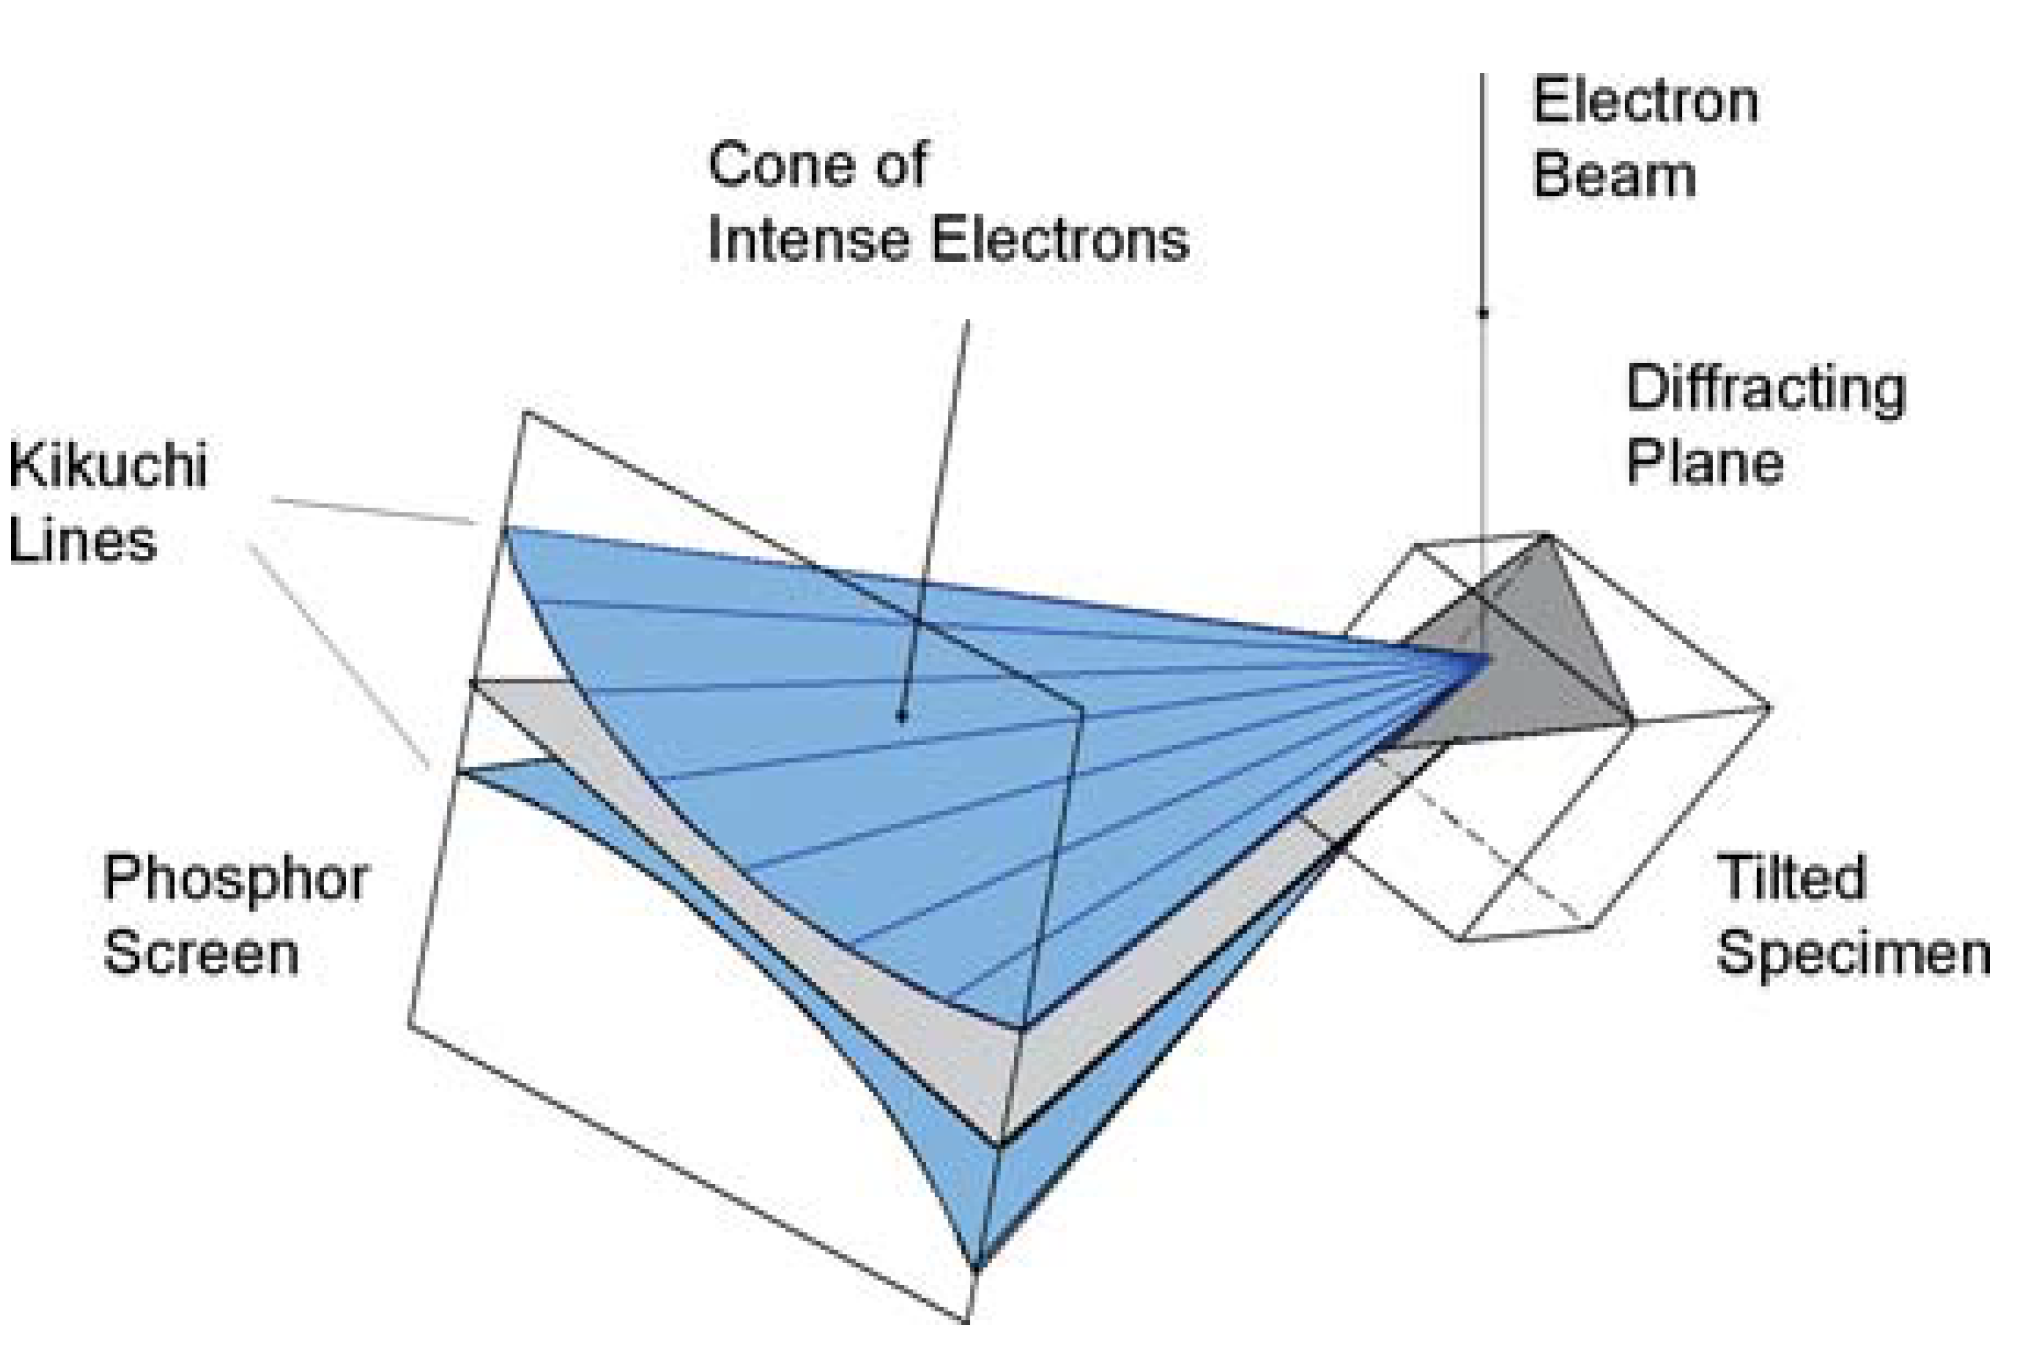
\includegraphics[width=0.6\textwidth]{img/ebsd_principle}
	\caption{The principle of electron backscatter diffraction. \cite{schwartz2009electron}.}
	\label{ebsd-principle}
\end{figure}

\begin{figure}
	
	\begin{subfigure}{.4\textwidth}
		\centering
		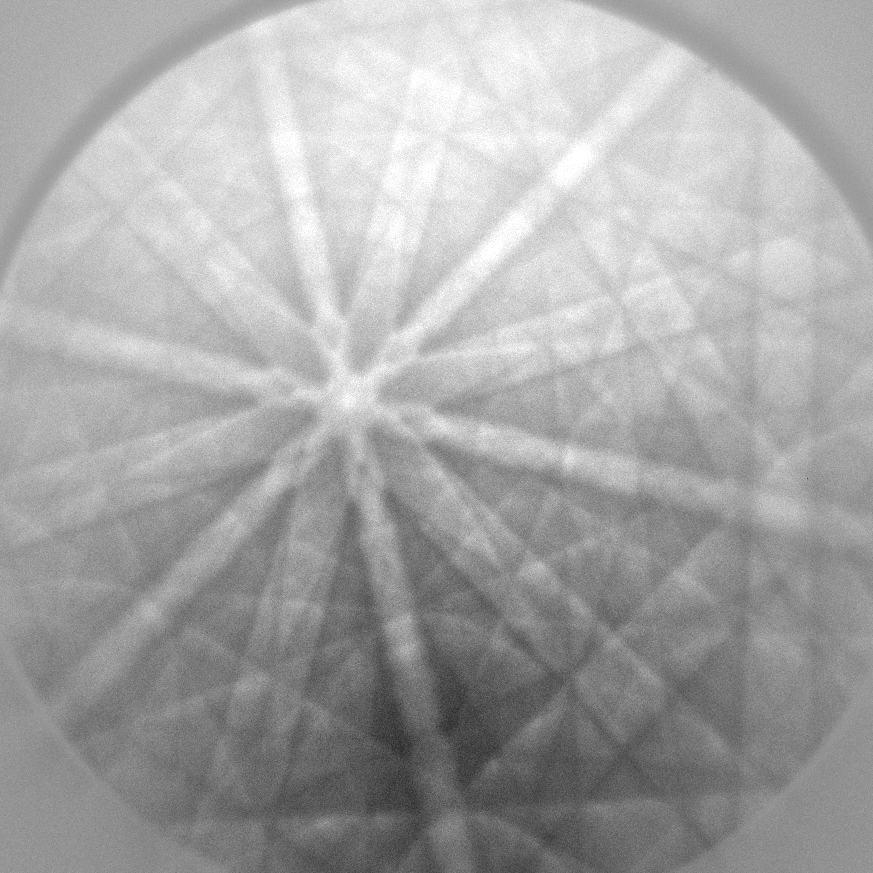
\includegraphics[width=.9\linewidth]{img/roi_shifts_initial}
		\caption{Initial, undeformed pattern}
		\label{roi-shifts:initial}
	\end{subfigure}%
	\begin{subfigure}{.4\textwidth}
		\centering
		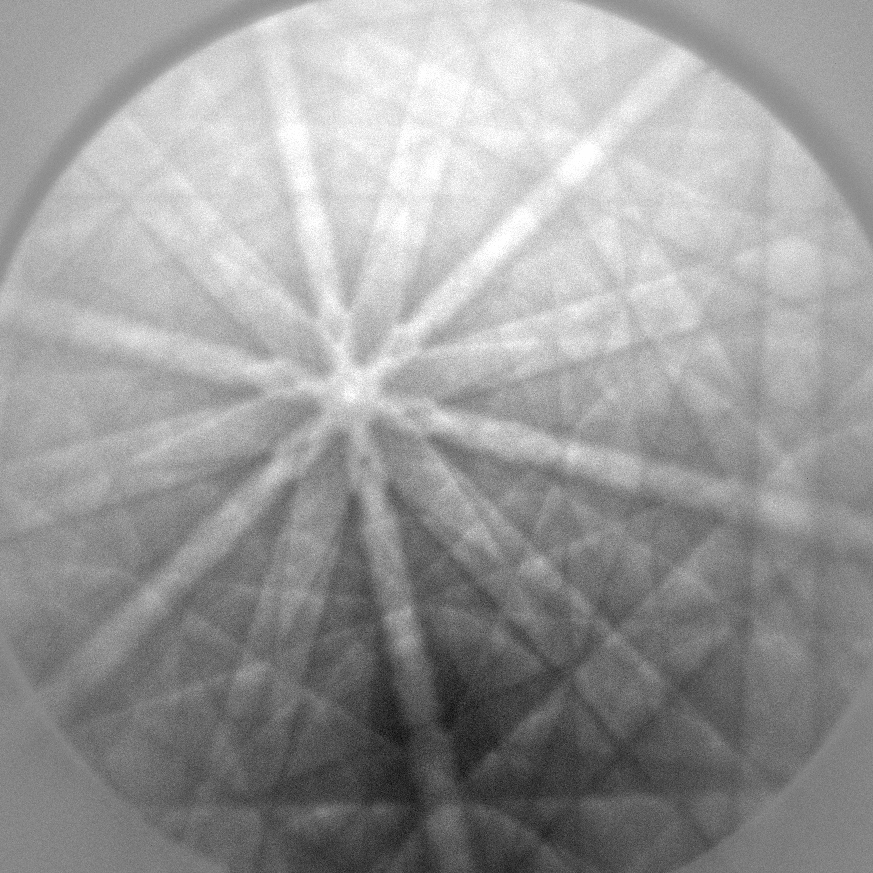
\includegraphics[width=.9\linewidth]{img/DEFORMED_x3600y6235}
		\caption{Deformed pattern}
		
	\end{subfigure}
	\centering
	\begin{subfigure}{.4\textwidth}
		\centering
		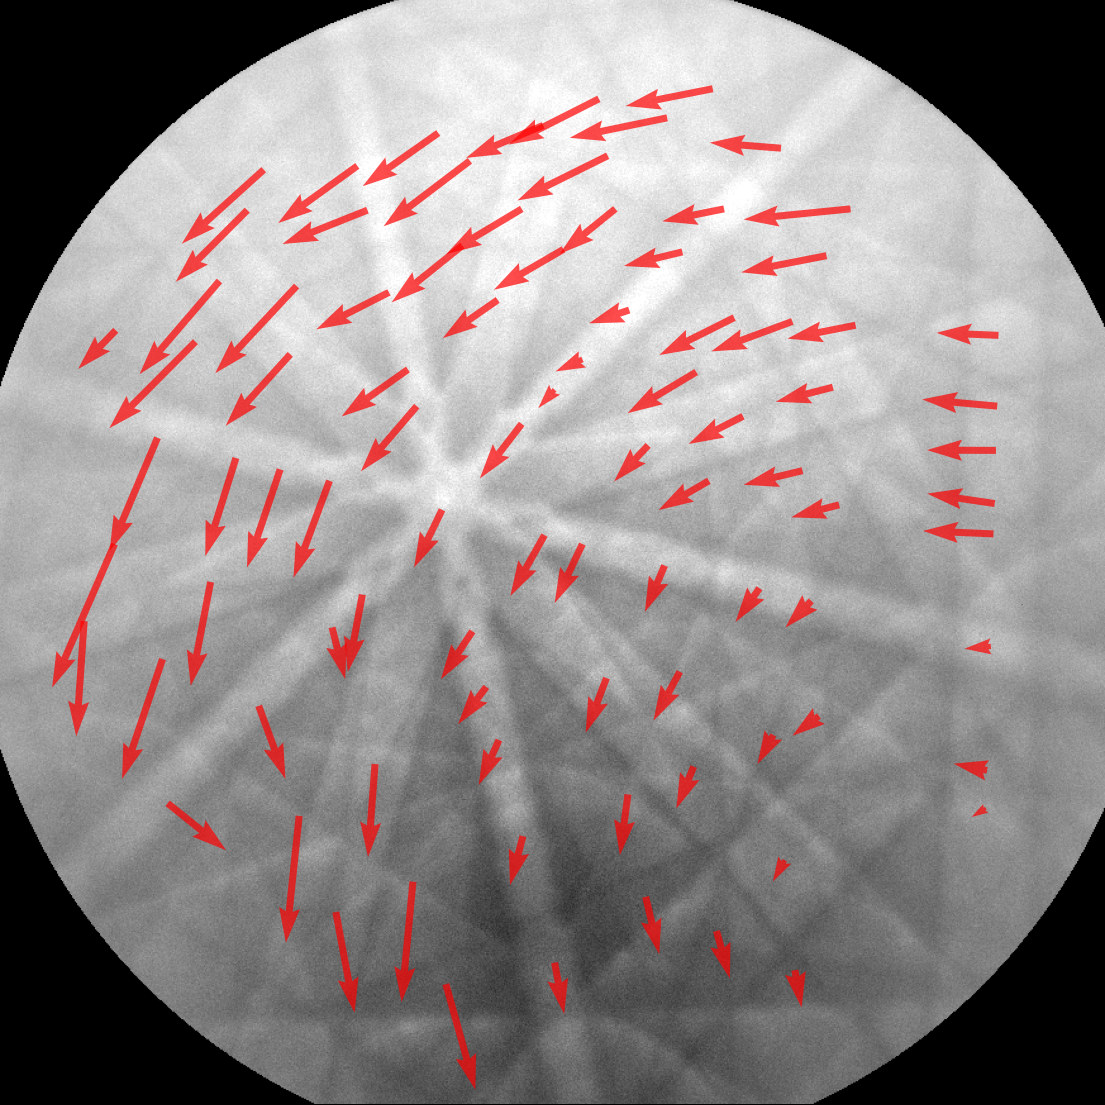
\includegraphics[width=.9\linewidth]{img/roi_shifts}
		\caption{Deformation visualization}
		\label{roi-shifts:result}
	\end{subfigure}
	
	\caption{Deformed pattern with arrows visualizing the deformation. The arrows are upscaled for the visualization, because the pattern is deformed only by several pixels (the biggest offset is less than 10 pixels long, while the whole picture has resolution $873 \times 873$).}
	\label{roi-shifts}
\end{figure}

The electrons do not reflect randomly, but based on the examined specimen, they backscatter in a specific way, forming \emph{Kukuchi lines} observable in the pattern. The geometry of Kukuchi lines can be interpreted as a projection of the specimen crystal structure on the flat phosphor screen.

When the crystal structure of material is changed (e.g. under stress), the deformation can be observed in the backscatter pattern as well. Therefore, the patterns of deformed specimen can be compared to undeformed ones to measure elastic strain and crystal lattice rotation.  \Cref{roi-shifts} shows a visualization of such comparison. Since different parts of the images may be deformed differently, a commonly used technique \cite{wilkinson2006high,wilkinson2010high,britton2012high} is to choose several (usually tens to hundreds) subregions of the patterns and determine the vector of shift between the corresponding regions from both patterns. The shifts estimate the real deformation of the crystalline structure.

The comparison is done by cross--correlating respective subregions of the deformed and reference patterns. The position of the maximum value in the correlation result determines the most probable shift with one pixel precision, which is not enough. To achieve subpixel accuracy, we estimate the peak of the cross--correlation by interpolating from a small neighborhood of the maximum.

Once the shifts are computed, they are further processed to obtain an estimation of the actual crystal deformation and other characteristics. However, we do not address that part of the analysis in this thesis, as it is not nearly as computationally expensive as the processing of the images. Moreover, the comparison is commonly used in analysis of the electron backscatter diffraction data, while the processing of the shifts may be different for various purposes.

To sum up, we have thousands images of deformed electron backscatter patterns. Each of them was captured by a scanning electron microscope at a specific location of a specimen. Moreover, we have one reference image of the electron backscatter pattern. We need to quantify the deformation of each deformed pattern, so we choose several subregions and cross--correlate each respective reference and deformed subregion. Maximal correlation gives us the most probable shifts of the subregions. So for each deformed pattern, the result of our algorithm is a list of shifts corresponding to subregions. The shifts are then further processed to obtain their physical interpretation, but that is not covered in this thesis.

%In this chapter we describe the algorithm used to analyze the deformation of the patterns. We define cross--correlation and least squares --- techniques that are used in the analysis. Finally, we describe the algorithm that we study in this thesis.

\section{Algorithm description}

In the rest of this chapter, we describe an algorithm used to process the electron backscatter patterns. The specifics of the algorithm correspond to a version that is used in Department of Physics of Material in Charles University in Prague.

The algorithm takes the following input and parameters:
\begin{itemize}
	\item reference image of electron backscatter pattern with size $W_p \times H_p$
	\item $N$ deformed images of electron backscatter pattern images, each with size $W_p \times H_p$
	\item $S$ positions of subregions that will be compared from each image
	\item size $W_s \times H_s$ of each subregion
	\item parameter $F$ that denotes the size of neighborhood used to interpolate the maximum with subpixel accuracy (see \cref{subpixel-peak})
\end{itemize}
The input images are all greyscale, which means each pixel is represented by one number. In our testing data, pixels were represented by 16 bit integers in range~$0 - 65535$.

The result of the algorithm is a list of $S$ shifts for each of the $N$ deformed patterns (see \cref{roi-shifts:result} for visualization of the shifts for one pattern).

Algorithm \ref{algo-whole-highlevel} shows a high--level pseudocode of the algorithm. It iterates through all deformed patterns and all subregion positions specified in the input. For each subregion, it computes the cross--correlation between the deformed subregion and subregion at the same position from the reference pattern. The result of cross--correlation is a matrix that expresses a measure of similarity for each possible shift between the subregions (see \cref{cross-corr-def}). In the next step, we further process the matrix to obtain the most probable shift with subpixel accuracy (see \cref{subpixel-peak}), which is the output of the algorithm.

\begin{algorithm}
	\caption{Processing of electron backscatter patterns}
	\label{algo-whole-highlevel}
	\KwIn{one reference electron backscatter pattern \newline
		$N$ deformed electron backscatter patterns \newline
		position of $S$ subregions from each pattern \newline
		size of a subregion \newline}
	\KwOut{deformation shifts for all $S$ subregions from all $N$ deformed patterns}
	\vspace{5px}
	
	refPat  $\leftarrow$ reference pattern\;
	\ForEach{\emph{defPat} in deformed patterns}{
		\ForEach{\emph{regPos} in subregion positions}{
			refReg, defReg $\leftarrow$ extract subregions from refPat and defPat\;
			
			crossResult $\leftarrow$ cross--correlate(refReg, defReg)\;
			
			maxX, maxY $\leftarrow$ subpixelPeak(crossResult)\;
			output [maxX, maxY]\;
		}
	}
\end{algorithm}

\section{Cross--correlation}
\label{cross-corr-def}
Cross--correlation provides a measure of similarity of two series for each possible shift between them. It is used in signal processing to find a shorter known feature in a signal or in image processing to locate a smaller shape in a bigger picture. In analysis of the backscatter patterns, it is used to find the most probable relative displacement between two images (subregions of images).

Cross--correlation of two discrete functions $f, g: \mathbb{Z} \rightarrow \mathbb{R}$ is a function $C:~\mathbb{Z} \rightarrow \mathbb{R}$ defined as follows:
\[
C[n] = (f \star g)[n] = \sum_{m=-\infty}^{\infty}f[m]g[m+n],
\]
where $\star$ denotes cross--correlation.

If $C = f \star g$ then $C[n]$ is a number that tells us how much are functions $f$ and $g$ similar, when $g$ is shifted by $n$ to the left. For each negative $n$, $g$ is shifted to the right. \Cref{correlation-example} shows two example functions and their cross--correlation.

\begin{figure}
	\centering
	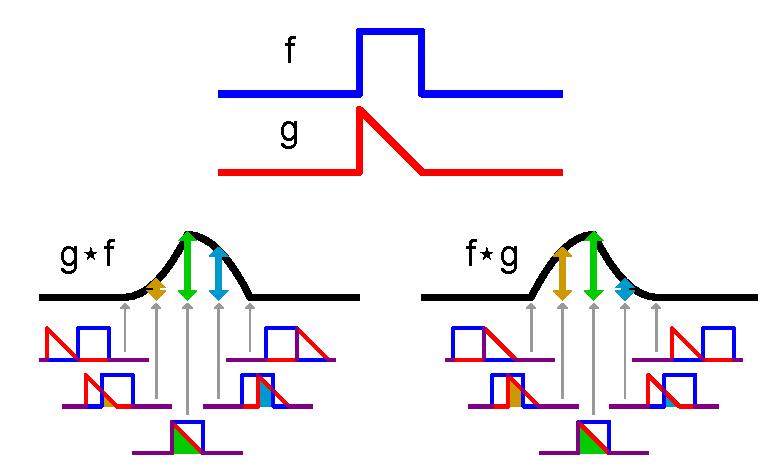
\includegraphics[width=0.7\linewidth]{img/correlation}
	\caption{The cross--correlation of two example functions\cite{correlation_example}.}
	\label{correlation-example}
\end{figure}

Definition of cross--correlation can be extended for two dimensions. For two--dimensional functions $f, g: \mathbb{Z}^2 \rightarrow \mathbb{R}$, their cross--correlation is a function $C: \mathbb{Z}^2 \rightarrow \mathbb{R}$ defined as:
\[
C[i,j] = (f \star g)[i,j] = \sum_{x=-\infty}^{\infty}\sum_{y=-\infty}^{\infty}f[x,y]g[x+i,y+j].
\]

Analogously to one--dimensional cross--correlation, $(f \star g)[i,j]$ is a number that is higher if $f$ is similar to $g$ shifted by $i$ horizontally and by $j$ vertically. \Cref{2d-correlation-example} demonstrates how cross--correlation can be used to search for a smaller pattern in a bigger picture. The brightest points (maxima) in \cref{2d-correlation-example-result} correspond to the best matches between the pattern and the image.

\begin{figure}[b!]
	\centering
		\begin{subfigure}{.49\textwidth}
		\centering
		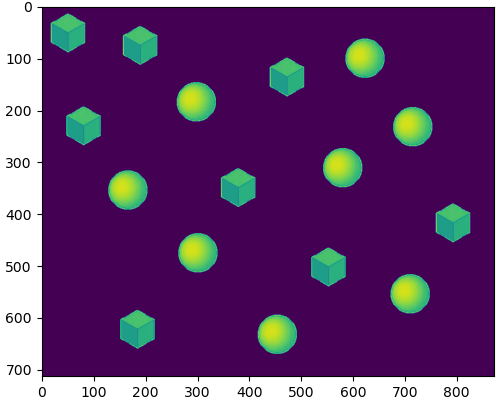
\includegraphics[width=\linewidth]{img/shapes}
		\caption{An image}
	\end{subfigure}
	\begin{subfigure}{.49\textwidth}
	\centering
	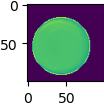
\includegraphics[width=0.4\linewidth]{img/shapes_pattern}
	\caption{Search pattern}
	%\label{fig:sub2}
	\end{subfigure}
	\begin{subfigure}{.5\textwidth}
		\centering
		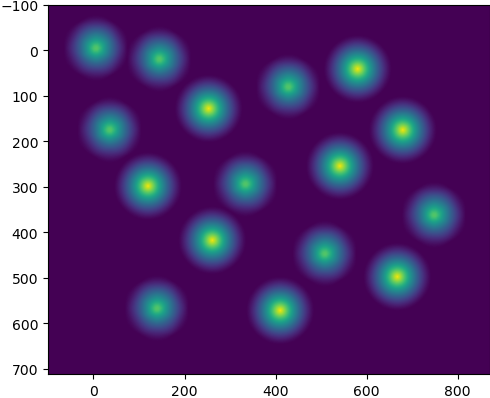
\includegraphics[width=\linewidth]{img/shapes_correlated}
		\caption{Cross--correlation of the (a) and (b) images}
		\label{2d-correlation-example-result}
	\end{subfigure}
	
	\caption{An example of cross--correlation used to find an object in an image. The maxima of the cross--correlation result correspond to the location of the search pattern (b) in the image (a).}
	\label{2d-correlation-example}
\end{figure}

Theoretically, the domain of cross--correlation is the whole $\mathbb{Z}^2$. However, when cross--correlating two images, i.e., real--valued matrices, $(f \star g)[i,j]$ does not make sense for all $[i,j] \in \mathbb{Z}^2$, because for some of them the images are shifted so much they do not overlap. For two images with sizes $w_1 \times h_1$ and $w_2 \times h_2$, the size of their relevant cross--correlation domain is $(w_1 + w_2 - 1) \times (h_1 + h_2 - 1)$. The result is a rectangle with the following corners: $[-w_1+1,-h_1+1]$, $[-w_1+1,h_2-1]$, $[w_2-1,h_2-1]$, $[w_2-1,-h_1+1]$. Those are the points of cross--correlation, where the result is computed from the images overlapping only by one pixel.

\subsection{Computing cross--correlation using discrete \\ Fourier transform}
\label{fft}

The cross--correlation can be computed using an algorithm based on its definition with asymptotic time complexity $\mathcal{O}(W_s^2H_s^2)$ for two images with resolution $W_s \times H_s$ --- for each of the resulting $(2W_s - 1)(2H_s - 1)$ pixels, we need to multiply at most $W_sH_s$ pixels. In the following section, we describe a way to compute two--dimensional cross--correlation in $\mathcal{O}(W_sH_s\log_2(W_sH_s))$ using \emph{discrete Fourier transform}. In the next section we show how it is used to compute \emph{circular cross--correlation}, which can be subsequently transformed into the (non--circular) cross--correlation we defined in the previous section.

%We first define \emph{circular cross--correlation}, because it can be used to compute cross--correlation. Then, we define \emph{discrete Fourier transform} and show how it is used to compute circular cross-correlation. Finally we show how to get the cross--correlation we need in the implementation. All is described for one--dimensional case only, since two--dimensional is analogous.

Let $N \in \mathbb{N}$, $\{x_n\} = x_0, x_1, \dots , x_{N-1}$ and $\{y_n\} = y_0, y_1, \dots , y_{N-1}$ be series of complex numbers. Then their circular cross--correlation is another series of $N$ numbers defined by the formula
\[
\{\mathbf{x} \star_N \mathbf{y}\}_n = \sum_{l=0}^{N-1}x^\star_ly_{(n+l)\bmod N},
\]
where $\cdot \star_N \cdot$ denotes the circular cross--correlation of two series.
%We can see that the definition is very similar to cross--correlation of two functions (see \cref{cross-corr-def}), except here we do.

Circular cross--correlation can be interpreted as a cross--correlation of two periodic functions. For any periodic function with period $N$, we only need $N$ consecutive values to represent, since the rest of the function repeats the same values. At the same time, given two periodic discrete functions $f, g : \mathbb{Z} \rightarrow \mathbb{C}$ with period $N$, their cross--correlation $f \star g$ is also periodic with the same period. So if we interpret the series in the definition of circular cross--correlation of as periodic functions, then the resulting series represents (non--circular) cross--correlation of the functions.

%The $\mod$ operation causes that whenever the $n+l$ is greater or equal than $N$, we ``circulate'' and take 

The circular cross--correlation can be quickly computed by using the discrete Fourier transform.

The \emph{discrete Fourier transform} is a function $\mathcal{F}: \mathbb{C}^N \times \mathbb{C}^N$ that transforms a series of $N \in \mathbb{N}$ complex numbers $\{x_n\} = x_0, x_1, \dots , x_{N-1}$ into another $N$ complex numbers $\{X_n\} = X_0, X_1, \dots , X_{N-1}$, which are defined as follows:
\[
X_k = \sum_{n=0}^{N-1} x_n \cdot e^{-\frac{i2\pi}{N}kn}.
\]
The Fourier transform is invertible, so if $\mathcal{F}(\mathbf{x}) = \mathbf{X}$, then $\mathcal{F}^{-1}(\mathbf{X}) = \mathbf{x}$.

Fourier transform has a broad range of practical applications --- it is used for example in digital signal processing, solving partial differential equations or big numbers multiplication. It can be used to quickly compute the circular cross--correlation using the following theorem \cite{proakis2004digital}.

Let $N \in \mathbb{N}$, $\{x_n\} = x_0, x_1, \dots , x_{N-1}$, $\{y_n\} = y_0, y_1, \dots , y_{N-1}$ be series of complex numbers and let $\{X_n\}$, $\{Y_n\}$ be their Fourier transforms. Then, we can compute \emph{circular cross--correlation} like so: 
\[
\mathcal{F}^{-1}\{\mathbf{X}^\star \cdot \mathbf{Y}\}_n = \sum_{l=0}^{N-1}x^\star_ly_{(n+l)\bmod N},
\]
where $\star$ denotes the \emph{complex conjugate} and $\cdot$ denotes element by element multiplication. Complex conjugate of a complex number $a + bi$, where $a, b \in \mathbb{R}$, is the complex number $a - bi$. Complex conjugate of series $\{a_n\}$ is series $\{b_n\}$, where every element $b_n$ is the complex conjugate of the original element $a_n$.

In other words, in order to compute the circular cross--correlation of two series $\{x_n\}$ and $\{y_n\}$, we first compute their Fourier transforms $\{X_n\}$ and $\{Y_n\}$, then multiply corresponding elements of $\{X_n\}$ and the complex conjugate of $\{X_n\}$. Finally, we do an inverse Fourier transform. We do all of this, because we are able to compute both the discrete Fourier transform and its inverse in time $\mathcal{O}(N \log N)$, which gives us the overall asymptotic time $\mathcal{O}(N \log N)$ compared to $\mathcal{O}(N^2)$ when computing the circular cross--correlation from definition.

%To compute non--circular cross--correlation using this method, we use a trick with zero padding. Let $N \in \mathbb{N}$, $f$ and $g$ be two discrete functions, that are non--zero only in the first 

\begin{figure}
	\centering
	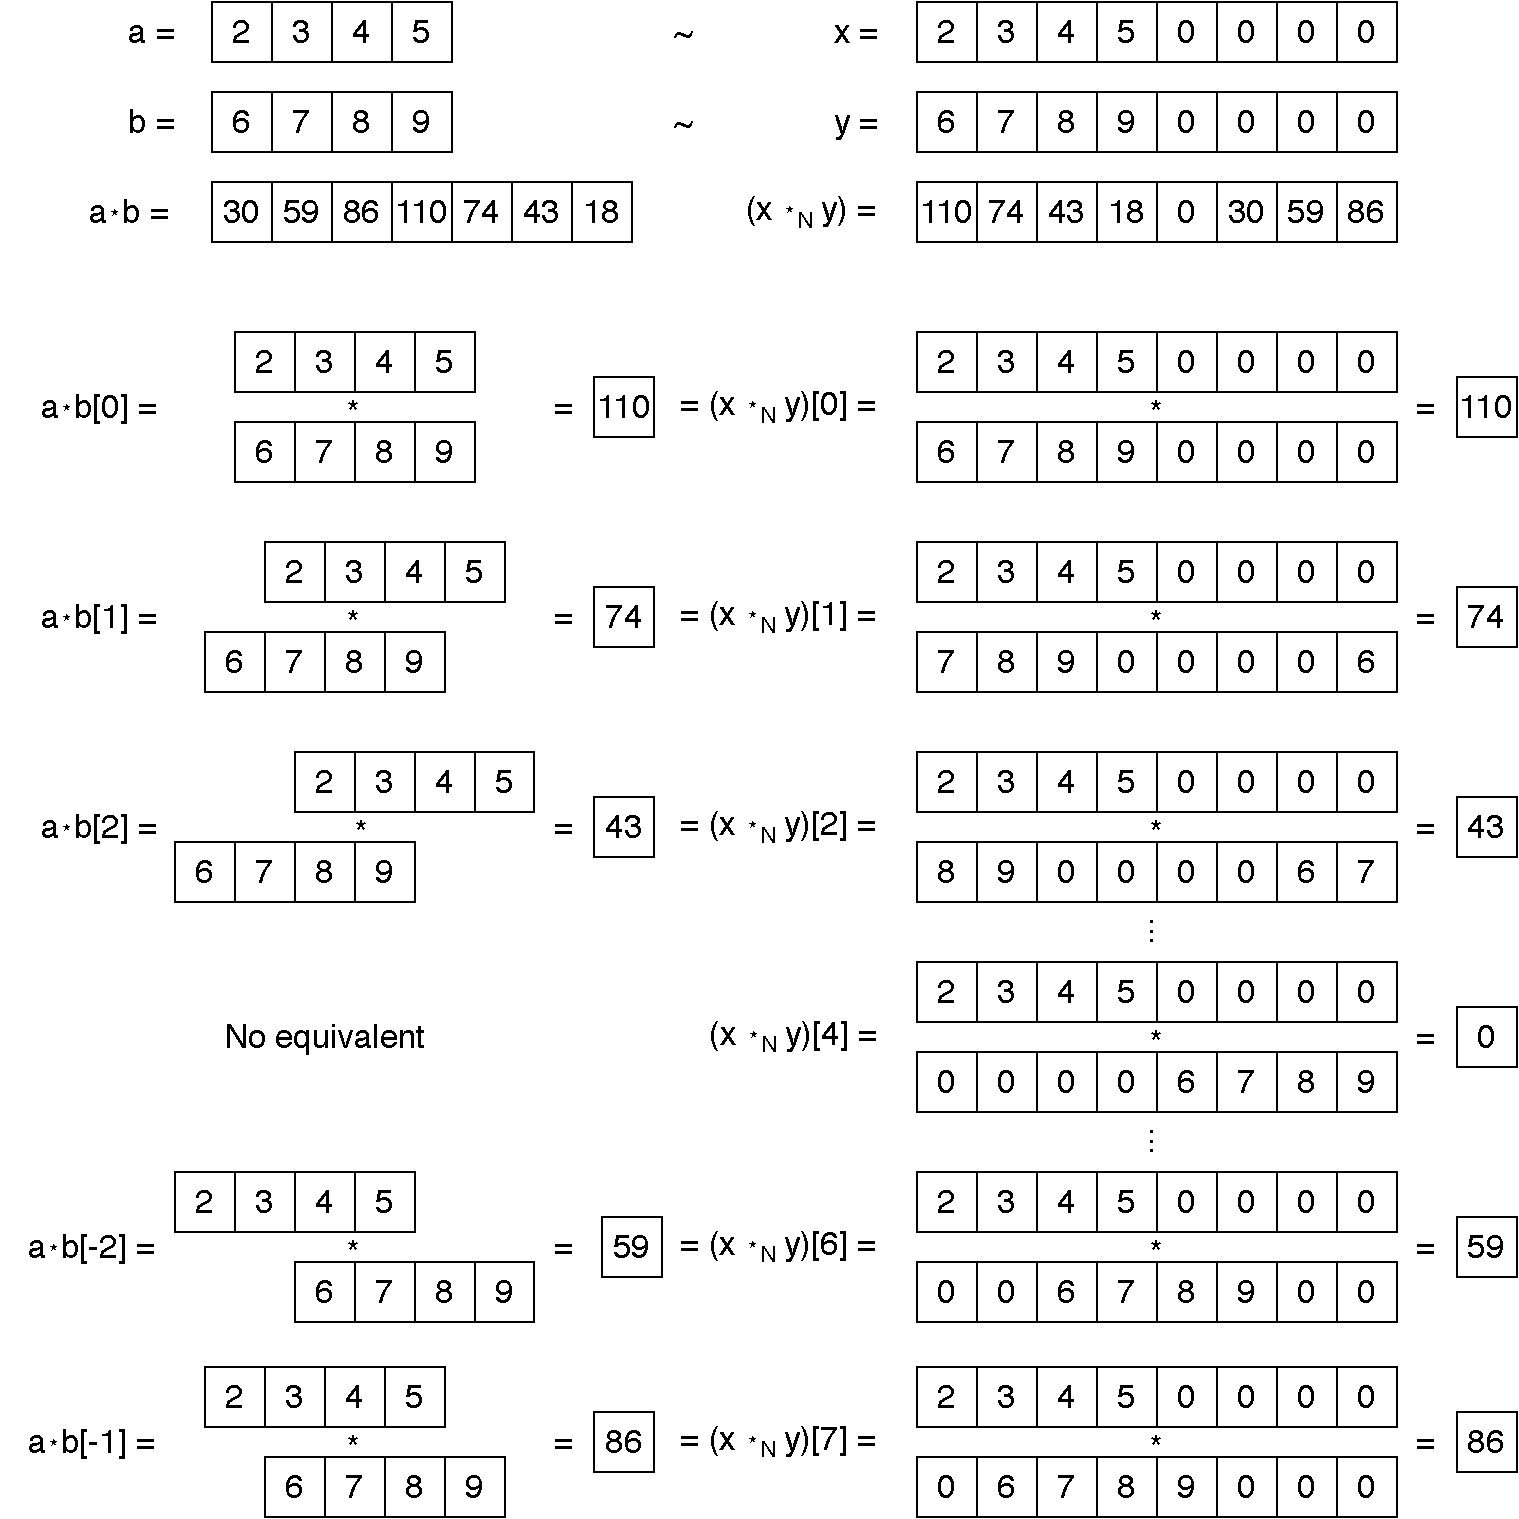
\includegraphics[width=\textwidth]{img/circ-cross-example}
	\caption{Illustration of the relationship between circular and non--circular cross--correlation. The left side shows a cross--correlation of two series $a$ and $b$. The right side shows the circular cross--correlation of $x$ and $y$, which are zero--padded versions of the series $a$ and $b$. Corresponding values of both correlations are shown side by side.}
	\label{circ-cross-example}
\end{figure}

To compute non--circular cross--correlation using this method, we use the following trick: for series $\{x_n\}$ and $\{y_n\}$ of length $N$, we expand both of them with $N$ zeros and then do circular cross--correlation. The result of such operation is the desired cross--correlation, only circularly shifted by N elements. The reason why it works is illustrated in \Cref{circ-cross-example}. When doing regular cross--correlation (in the left side of the figure), we slide one of the series along the other and for every shift, we multiply the corresponding numbers. If a number does not have any counterpart in the other series with respect to the current shift, it is discarded. For circular cross--correlation, we again slide one of the series, but this time we do it circularly using the modulo operator. We use the zeros that we expanded the original series with to rule out the values that should not be multiplied for the current shift.

The circular cross--correlation of zero--padded series results in a series $\{c_n\} = \mathbf{x} \star_N \mathbf{y}$ of $2N$ numbers. The numbers in the series have the following interpretation: $c_0, \cdots, c_{N-1}$ are the values of non--circular cross--correlation with shifts $0, 1, \cdots, N$ and $c_{N+1}, c_{N+2}, \cdots, c_{2N-1}$ represent the shifts $(-N+1), (-N+2), \cdots, -2, -1$. $c_{N}$ is always zero and does not have any interpretation.

\subsubsection{Two--dimensional discrete Fourier transform}
\label{two-dim-ft}
In order to use the described method in our implementation, we need to expand it to work on two--dimensional inputs.

Let $N, M \in \mathbb{N}$, $\mathbf{x} \in \mathbb{C}^{N\times M}$. Then $\mathbf{X} \in \mathbb{C}^{N\times M}$ is the Fourier transform of x, if the following holds for each item of the matrix $\mathbb{X}$:
\[
X_{k,l} = \sum_{n=0}^{N-1} \sum_{m=0}^{M-1} x_{n,m} \cdot e^{-i2\pi(\frac{kn}{N} + \frac{lm}{M})}.
\]

Next, the circular cross--correlation theorem can be rewritten for two dimensions as well. Let $N, M \in \mathbb{N}$, $\mathbf{x} \in \mathbb{C}^{N\times M}$, $\mathbf{y} \in \mathbb{C}^{N\times M}$ let $\mathbf{X} = \mathcal{F}(\mathbf{x})$ and $\mathbf{Y} = \mathcal{F}(\mathbf{y})$ be their Fourier transforms. Then, we can compute the two--dimensional circular cross--correlation like so: 
\[
\mathcal{F}^{-1}\{\mathbf{X}^\star \cdot \mathbf{Y}\}_{n,m} = \sum_{k=0}^{N-1} \sum_{l=0}^{M-1} x^\star_{k,l} y_{(n+k)\bmod N, (m+l)\bmod M},
\]
where $\cdot^\star$ denotes the complex conjugate and $\cdot$ denotes element by element multiplication.

The trick with zero--padding the inputs applies to the two--dimensional case as well. So when we want to compute the cross--correlation of two images $x$ and $y$ (represented by matrices in the theorem) with resolution $W \times H$, we do the following steps:
\begin{enumerate}
	\item Zero--pad the images --- we enlarge the image to the size $2W \times 2H$ by adding zeros.
	\item Compute the Fourier transforms of the images, which gives us two matrices $X = \mathcal{F}(x)$ and $Y =\mathcal{F}(y)$ of complex numbers with sizes $2W \times 2H$.
	\item Compute the complex conjugate of the matrix $X$.
	\item Multiply $X^\star$ with $Y$ element by element. The operation is also called \emph{Hadamard product}.
	\item Do the inverse discrete Fourier transform on the product.
\end{enumerate}
The result is a matrix $R$ of real numbers with the size $2W \times 2H$. It contains the cross--correlation of the input images, but it is circularly shifted. Similar to the one--dimensional case, where the item $N$ of the series was always zero, now the column $R_{*,N}$ and row $R_{N,*}$ are both zero. They separate the matrix into 4 quadrants that are circularly shifted by $N$ compared to the cross--correlation. Thus, the last step needed to get the resulting cross--correlation is to shift the matrix back by $N$, which is the same as swapping the quadrants diagonally.

\subsection{Zero--normalized cross--correlation}

Cross--correlation as we defined it (see \cref{cross-corr-def}) has a major flaw for image processing: it is heavily affected by the brightness of the images. Consider an image, that has some subregions brighter than others. Then, by definition of cross--correlation, that subregions add more to the result, regardless of the second image. \Cref{normalized-initial} shows an example of an image that is much brighter in the top part than in the bottom. \Cref{normalized-simple-cross} shows the result of cross--correlation with the search pattern in \cref{normalized-pattern}. It is clear that the highest values are located where the original image is brightest instead of locating the search pattern.

\begin{figure}
	\centering
	\begin{subfigure}{.5\textwidth}
		\centering
		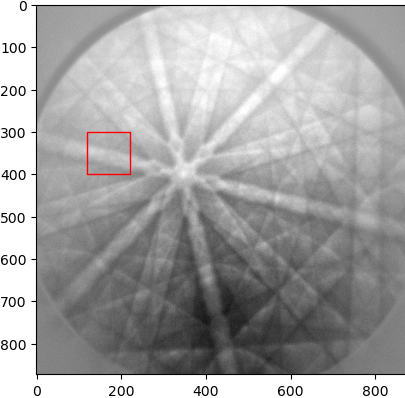
\includegraphics[width=\linewidth]{img/normalized_initial}
		\caption{An electron backscatter pattern}
		\label{normalized-initial}
	\end{subfigure}
	\begin{subfigure}{.4\textwidth}
		\centering
		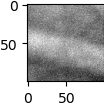
\includegraphics[width=0.4\linewidth]{img/normalized_pattern}
		\caption{Search pattern}
		\label{normalized-pattern}
	\end{subfigure}
	\begin{subfigure}{.49\textwidth}
		\centering
		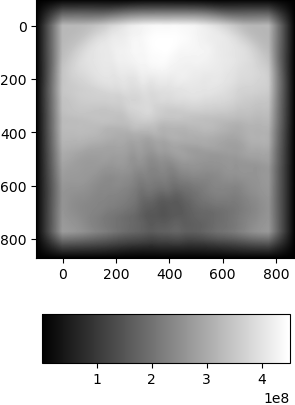
\includegraphics[width=\linewidth]{img/normalized_simple_corr}
		\caption{Simple cross--correlation of the (a) and (b) images}
		\label{normalized-simple-cross}
	\end{subfigure}
	\begin{subfigure}{.49\textwidth}
		\centering
		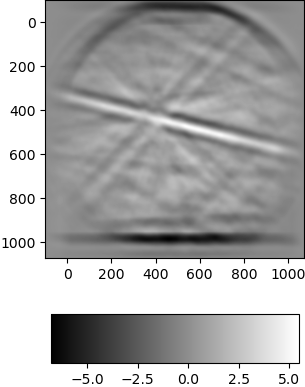
\includegraphics[width=\linewidth]{img/normalized_corr}
		\caption{Normalized cross--correlation of the (a) and (b) images}
		\label{normalized-cross}
	\end{subfigure}
	
	\caption{A comparison between the simple and zero--normalized cross--correlation. An image of backscatter pattern (a) is correlated with its subregion (b). (c) shows that simple cross--correlation is affected by varying brightness in different parts of images. (d) shows that normalization of the images improve the cross--correlation results.}
\end{figure}

That is why zero--normalized cross--correlation is used. It is based on subtracting respective means from each image. Normalized cross--correlation of two images $f$ and $g$ is defined as follows:
\[
\textsc{ZNCC}[i,j] = \sum_{x, y} \frac{1}{\sigma_f \sigma_g}(f[x,y] - \mu_f)(g[x+i,y+j] - \mu_g),
\]  
where $\mu_f$ and $\mu_g$ are the means of the images and $\sigma_f$, $\sigma_g$ are their standard deviations. For an image $f$ with size $W \times H$, they are defined as follows:
\begin{align*}
\mu_f &= \frac{1}{WH} \sum_{x,y}{}f[x,y], \\
\sigma_f &= \sqrt{\frac{1}{WH-1} \sum_{x,y}(f[x,y]-\mu_f)^2}.
\end{align*}

\Cref{normalized-cross} shows the zero--normalized cross--correlation of the figures \ref{normalized-initial} and \ref{normalized-pattern}. The area of the highest correlation is now clearly visible and corresponds to a Kukuchi line in the original image. Subtracting the mean of both images makes the algorithm less prone to brightness changes across the image.

The intuition behind this behavior is as follows. By the definition of simple cross--correlation, pixels with low brightness multiply and result in low correlation. After subtracting the means, low values in both images become negative. However, two negative numbers multiply into a positive value, so they increase the correlation. On contrary, very bright and very dark pixels multiply into a negative number so their difference causes that they lower the overall correlation value.

The zero--normalized cross--correlation is used in processing of the electron backscatter patterns to compare the reference deformed subregions. It can be computed in three steps:
\begin{enumerate}
	\item Find the means of the reference and deformed subregions
	\item Subtract the means from the pixels of both subregions
	\item Find the standard deviations of the reference and deformed subregions
	\item Divide the the pixels of both subregions by their respective standard deviations
	\item Compute the cross--correlation of the subregions
\end{enumerate}
First four steps normalize the subregions and then we perform the simple two--dimensional cross--correlation. The result is a two--dimensional matrix with size $(2W_s-1) \times (2H_s-1)$, if the subregions have size $W_s \times H_s$.


\section{Subpixel peak}
\label{subpixel-peak}
Next, we find the maximum of the cross--correlation. The location of the maximum $[x_m,y_m]$ in the matrix is the shift between the deformed and reference subregions. However, the precision of one pixel is not accurate enough in the context of the nanoworld the electron backscatter diffraction studies. That is why we use the cross--correlated data to estimate the maximum with subpixel accuracy.

We expect that if we could compute the cross--correlation with infinite resolution, so it would be continuous, the neighborhood of the maximum would look like a two--dimensional quadratic function with exactly one maximum. Since we only have limited resolution, we estimate~(fit) the continuous quadratic function from several discrete points of the cross--correlation --- the neighborhood of the maximum. The neighborhood is square--shaped and its size $F \times F$ is a parameter of the algorithm. Finally, we find the exact location of maximum of the estimated continuous quadratic function, which may be slightly shifted from the discrete maximum, depending on the values of the cross--correlation in the neighborhood.


So the processing of the cross--correlation is done in several steps:
\begin{enumerate}
	\item Find the position $[x_m,y_m]$ of the maximum (often denoted as \emph{arg max} operation) of the cross--correlation. It is a pair of whole numbers from the closed interval $(-W_s, W_s) \times (-H_s, H_s)$.
	\item Use the \emph{least squares method} to fit a quadratic function to the neighborhood of the maximum. The function is a continuous representation of the cross--correlation peak.
	\item Find the position of the maximum of the continuous function.
\end{enumerate}

In the following sections, we describe these steps in detail.

\subsection{Least squares}
The least squares method is used to approximate the solution of systems of equations which do not have an exact solution, since there are more equations than variables. Such systems are also called overdetermined systems. In the electron backscatter pattern analysis, the least squares method is used to approximate coefficients of a quadratic function from its several known points.

In the first place, let us formulate the problem that the least squares method addresses. Let $n,m \in \mathbb{N}, n > m; A \in \mathbb{R}^{n \times m}; x \in \mathbb{R}^m$ and $b \in \mathbb{R}^n$. Then $Ax = b$ is an overdetermined system of linear equations. It may have a solution, if $b$ is a linear combination of column vectors of $A$ ($b$ is in column space of $A$), but in general, that is not the case.

Instead of solving the system, we search for a vector $x'$ that has the least difference from the right hand side of the equation:
\[
x' = \min_x \norm{Ax - b},
\]
where $\norm{\cdot}$ denotes Euclidean norm. For a vector $x \in \mathbb{R}^n$, it is defined as:
\[
\norm{x} = \sqrt{\sum_{i=0}^{n} x_i^2}.
\]
So we minimize the sum of squared differences between the left and right sides of the equations in the system, hence the name least squares.

The least squares solution can be calculated using only matrix multiplication and inversion as follows \cite{anton2013elementary}:  
\[
x' = (A^TA)^{-1}A^Tb.
\]

This formula is not used in practice because of effectiveness and numerical stability (instead, it is better to solve the equation $A^TAx = A^Tb$). However, for the algorithm described in this thesis, the approach is sufficient, since the matrix $A$ is constant in our case (as we will explain in the end of \cref{estimation} for further explanation).

\subsection{Maximum neighborhood fitting}

We use the least squares method to estimate the coefficients of a two--dimensional quadratic function from the neighborhood of the cross--cor\-re\-la\-tion maximum. The neighborhood has size $F \times F$ and has the shape of a square, so for maximum at location $[x_m, y_m]$, the neighborhood points are at positions 
\[
\{x_m - \frac{F-1}{2}, \cdots, x_m, \cdots, x_m + \frac{F-1}{2}\} \times \{y_m - \frac{F-1}{2}, \cdots, y_m, \cdots, y_m + \frac{F-1}{2}\}.
\]
We only consider odd $F$, so the maximum is always in the middle.

The estimated two--dimensional quadratic function $f:\mathbb{R} \rightarrow \mathbb{R}$ can be written as as:
\[
f(x,y) = a + bx + cy + dx^2 + exy + fy^2,
\]
where $a, b, c, d, e, f \in \mathbb{R}$. To estimate such function is to find the 6 coefficients $a \dots f$. From the known points of the neighborhood $N$ of size $F \times F$, it is possible to create the following system of equations:
\[
\forall [x,y] \in \{0,1,\dots , F-1\}^2 : a + xb + yc + x^2d + xye + y^2f = N[x,y],
\]
where $a \dots f$ are unknown variables.

So for each point with coordinates $[x,y]$ in the neighborhood, we create one equation with substituted $x$ and $y$. We have $F^2$ known points, from which we create $s^2$ equations. We have 6 unknown variables and $F$ has to be greater than one and odd, so we have more equations than unknowns. 

\subsubsection{Example of creating equation system}

For instance, let $F$ be 3 and $N$ be the neighborhood of the maximum:
\[
N =
\begin{bmatrix}
751 & 819 & 765 \\
825 & 934 & 810 \\
768 & 798 & 725
\end{bmatrix}.
\]


\iffalse
\[
\begin{bmatrix}
1 & 0 & 0 & 0 & 0 & 0\\
1 & 1 & 0 & 1 & 0 & 0\\
1 & 2 & 0 & 4 & 0 & 0\\
1 & 0 & 1 & 0 & 0 & 1\\
1 & 1 & 1 & 1 & 1 & 1\\
1 & 2 & 1 & 4 & 2 & 1\\
1 & 0 & 2 & 0 & 0 & 4\\
1 & 1 & 2 & 1 & 2 & 4\\
1 & 2 & 2 & 4 & 4 & 4
\end{bmatrix}
\cdot
\begin{bmatrix}
a \\ b \\ c \\ d \\ e \\ f
\end{bmatrix}
=
\begin{bmatrix}
751 \\ 819 \\ 765 \\ 825 \\ 934 \\ 810 \\ 768 \\ 798 \\ 725
\end{bmatrix}.
\]
\fi

Then, the linear system looks like this:
\begin{align*}
x=0,y=0 \rightarrow a + 0b + 0c + 0d + 0e + 0f &= N[0,0] = 751 \\
x=1,y=0 \rightarrow a + 1b + 0c + 1d + 0e + 0f &= N[1,0] = 819 \\
x=2,y=0 \rightarrow a + 2b + 0c + 4d + 0e + 0f &= N[2,0] = 765 \\
x=0,y=1 \rightarrow a + 0b + 1c + 0d + 0e + 1f &= N[0,1] = 825 \\
x=1,y=1 \rightarrow a + 1b + 1c + 1d + 1e + 1f &= N[1,1] = 934 \\
x=2,y=1 \rightarrow a + 2b + 0c + 4d + 2e + 1f &= N[2,1] = 810 \\
x=0,y=2 \rightarrow a + 0b + 2c + 0d + 0e + 4f &= N[0,2] = 768 \\
x=1,y=2 \rightarrow a + 1b + 2c + 1d + 2e + 4f &= N[1,2] = 798 \\
x=2,y=2 \rightarrow a + 2b + 2c + 4d + 4e + 4f &= N[2,2] = 725 \\
\end{align*}

The left sides contains the equation of the two--dimensional quadratic function with substituted points from the set $\{0,1,2\}^2$ (for this example, we have chosen the zero point to be the top left corner). The right side contains all the corresponding values from neighborhood $N$.

\subsubsection{Estimation of function coefficients using least squares method}
\label{estimation}

Once we create the system of equations, we solve it using the least squares method. Recall its solution:
\[
x' = (A^TA)^{-1}A^Tb.
\]
Matrix $A$ in the solution corresponds to the left sides of the system of equations, $b$ is the vector with values of the neighborhood. We can observe that the left sides of the equations (matrix $A$) are constant for any neighborhood of size $F$. That also implies that the expression $(A^TA)^{-1}A^T$ in the least squares solution is constant for the values of the neighborhood and only depends on the parameter $F$.

That means we can precompute the constant part of the least squares formula for each $F$. That reduces the computation of least squares to only one matrix--vector multiplication. We do not expect that $F$ can have many different values. It has to be odd and the neighborhood is expected to be fairly small --- for this thesis we implemented only the options $F \in \{3, 5, 7, 9\}$.


\subsection{Maximum of fitted function}
\label{max-fitted}
The last step in the algorithm is to find the maximum of the quadratic function. We do that using standard methods of mathematical analysis: we find where are the partial derivations of the function equal to zero.

The partial derivations of the quadratic function are:
\begin{align*}
\frac{\partial f}{\partial x}(x,y) &= 2dx + ey + b,\\
\frac{\partial f}{\partial y}(x,y) &= ex + 2fy + c.
\end{align*}

If the function has an extreme, then it is located at the point where the partial derivations are both zero. That implies a linear system of equations with the following solution:
\begin{align*}
x_m &= \frac{2bf - ce}{e^2 - 4df}\\
y_m &= \frac{2cd - be}{e^2 - 4df}
\end{align*}

The point $[x_m, y_m]$ is the maximum of the function fitted to the neighborhood of the cross--correlation maximum.

\subsubsection{Scaling the neighborhood by constant}

When we multiply the result of the cross--correlation by constant, the result of the algorithm does not change. The reason is as follows. In the first step of the algorithm, we find the position of maximum of the cross--correlation which is not affected by constant scaling. Next, since the neighborhood is scaled by constant, the quadratic function approximation will be scaled as well. Finally, we find the maximum position of the estimated continuous function, which is the same as if the function was not scaled.

It means that when computing the zero--normalized cross--correlation, we can omit two of its steps --- computation of standard deviation and division by the result, which simplifies the final algorithm.

\section{Summary}
\label{algo-summary}
Algorithm \ref{algo-whole} summarizes the algorithm described in this chapter. It is clear that all the patterns and even their subregions are processed separately so it is easy to parallelize it. At the same time, there may be thousands of the patterns and tens of subregions in each, so there is enough data to utilize the whole GPU. The most computationally expensive part is the cross--correlation. We explain the implementation details of the algorithm in the next chapter.

\begin{algorithm}
	\caption{EBSP deformation processing}
	\label{algo-whole}
	\KwIn{one reference electron backscatter pattern \newline
		$N$ deformed electron backscatter patterns \newline
		position of $M$ subregions from each pattern \newline
		size of a subregion \newline
		parameter $F$ --- size of neighborhood}
	\KwOut{deformation shifts for all $M$ subregions from all $N$ deformed patterns}
	\vspace{5px}
	
	refPat  $\leftarrow$ load reference pattern from disk\;
	\ForEach{deformed pattern}{
		defEBSP $\leftarrow$ load deformed pattern from disk\;
		\ForEach{\emph{regPos} in subregion positions}{
			refReg $\leftarrow$ extract subregion at regPos from refPat\;
			defReg $\leftarrow$ extract subregion at regPos from defPat\;
			\BlankLine
			refMean, defMean $\leftarrow$ means of both subregions\;
			\BlankLine
			subtract refMean from pixels of refReg\;
			subtract defMean from pixels of defReg\;
			\BlankLine
			crossResult $\leftarrow$ cross--correlate(refReg,defReg)\;
			\BlankLine
			maxX, maxY $\leftarrow$ subpixelPeak(crossResult)\;
			output [maxX, maxY]\;
		}
	}
	
	\SetKwProg{Fn}{Function}{}{end}
	\SetKwFunction{FSubpixelPeak}{subpixelPeak}    
	\Fn{\FSubpixelPeak{crossResult}}{
		[maxX, maxY] $\leftarrow$ argmax(crossResult)\;
		neighbors $\leftarrow$ extract neighborhood of [maxX, maxY]\;
		
		coefs $\leftarrow$ fitQuadraticFunction($F$, neighbors)\;
		\KwRet arg max of the quadratic function with coefficients coefs \;
	}
\end{algorithm}


%\subsection*{How to build}
The project uses the CMake build system.

\vspace{0.3cm}
\noindent
Requirements:
\begin{itemize}
	\item git
	\item CMake version at least 3.9
	\item C++17 compiler (tested on MSVC from Visual Studio 16.8, GCC 8.3 and GCC 9)
	\item CUDA compute capability: 6.0
\end{itemize}
Tested on 2 platforms so far:
\begin{itemize}
	\item Windows - Visual Studio 2019, CUDA 10.2
	\item Linux - GCC 8.3, CUDA 10.2
\end{itemize}

\subsubsection*{Windows}

\begin{enumerate}
	\item Open the project folder in Visual Studio. It should detect CMake project and start configuration.
	\item Choose the x64-Release configuration.
	\item Build $\rightarrow$ Build all (F6)
	\item The resulting executable emida.exe is in \texttt{build/x64-Release/bin} folder.
\end{enumerate}
You may also run \texttt{build/x64-Release/bin/emida\_test.exe} to verify the build.

\subsubsection*{Linux}

On linux, it is preferred to use system libtiff (it is downloaded and built from source on Windows). Alternatively, there is \texttt{TIFF\_FROM\_SOURCE} switch that enforces building libtiff from source, but ZLIB and LibLZMA packages are still required by the libtiff library. The following steps are an example how to build the project on Ubuntu. We assume that a compatible C++17 compiler is set as default.
\begin{enumerate}
	\item Install the libtiff, cmake and git packages: 
	\begin{verbatim}
	apt-get install -y cmake git libtiff-dev
	\end{verbatim}
	\item Run the following in the terminal from the project folder.
	\begin{verbatim}
	mkdir build && cd build
	cmake ../
	cmake --build .
	\end{verbatim}
	\item The resulting executable emida is in \texttt{build/bin} folder.
\end{enumerate}
You may also run \texttt{bin/emida\_test} to verify the build.

\subsection*{How to run}

The application compares one picture of the material patern with images of deformed material. The deformed images are specified by an input file that has lines in following format:
\begin{verbatim}
<image_pos_x> <image_pos_y> <image_file_name>
\end{verbatim}
Example:
\begin{verbatim}
0.0 0.0 E:/emida/data/FeAl/DEFORMED_FeAl/DEFORMED_x0y0.tif
600.0 0.0 E:/emida/data/FeAl/DEFORMED_FeAl/DEFORMED_x600y0.tif
1200.0 0.0 E:/emida/data/FeAl/DEFORMED_FeAl/DEFORMED_x1200y0.tif
1800.0 0.0 E:/emida/data/FeAl/DEFORMED_FeAl/DEFORMED_x1800y0.tif
300.0 519.6152422706632 E:/emida/data/FeAl/DEFORMED_FeAl/DEFORMED_x300y519.tif
900.0 519.6152422706632 E:/emida/data/FeAl/DEFORMED_FeAl/DEFORMED_x900y519.tif
\end{verbatim}
Positions and size of regions that are compared in each picture are specified in a configuration file in fillowing format:
\begin{verbatim}
<size/2>\n
<roi_mid_x> <roi_mid_y>\n
<roi_mid_x> <roi_mid_y>\n
...
\end{verbatim}
The size of each region is specified on the first line. The size is half ("radius") of the compared regions. Then, list of pairs follow, each of them specifies a middle of one subregion.

\subsubsection*{Running emida}
The \texttt{emida} executable cross-correlates parts of pictures(slices) in specified positions and then computes how much are the deformed picture's slices shifted compared to the initial picture.
\begin{verbatim}
emida -i data/FeAl/INITIAL_FeAl -d data/FeAl/DEFORMED_FeAl \
-o data/FeAl/OUT_FeAl -r 0,0,5,5 -c 25,25 -s 64,64 > offsets.txt
\end{verbatim}
Following options are mandatory:
\begin{itemize}
	\item \texttt{-i,--initial} specifies path to the reference image
	\item \texttt{-d,--deformed} specifies path to file with list of the deformed pictures to process. The format of the file is described above.
	\item \texttt{-b,--slicepos} specifies path to file with positions of regions to be compared in each picture, as descibed above.
\end{itemize}
Optional options:
\begin{itemize}
	\item \texttt{-s,--slicesize} overrides the size of subregions specified in the subregion description passed by the \texttt{slicepos} parameter.
	\item \texttt{-q,--writecoefs} In addition to offsets, output also coefficients of parabola fitting.
	\item  \texttt{--precision} specifies the floating type to be used. Allowed values: \texttt{double}, \texttt{float}.
	\item \texttt{f,fitsize} specifies the size of neighbourhood that is used to fit the quadratic function to cross--correlation and find subpixel maximum. Allowed values: 3, 5, 7, 9
	\item \texttt{crosspolicy}, Specifies whether to use FFT to compute cross correlation. Allowed values: brute, fft.
	\item \texttt{batchsize}, Specifies how many files are processed in one batch in parallel.
	\item \texttt{loadworkers}, Specifies the number of workers that load input patterns simultaneously.
	\item \texttt{-a} When specified, the executable measures the duration of selected kernels and parts of processing.
\end{itemize}

\subsubsection*{Running emida}

The package contains testing data in the \texttt{test\_data} folder. \texttt{test\_data/initial} contains the reference, unmodified pattern. \texttt{test\_data/deformed} contains the deformed patterns. Due to limited options of uploading large attachments, we attached only a subset of original testing data. \texttt{test\_data/def.txt} contains list of the files in the format described above that can be loaded by the executable.

\vspace{0.3cm}
\noindent
The deformed images have file names in the following format:
\begin{verbatim}
DEFORMED_x<X_position>y<X_position>.tif
\end{verbatim}
The \texttt{X\_position} and \texttt{Y\_position} are integers that determine the position where the pattern was measured on the studied specimen.

\vspace{0.3cm}
\noindent
The patterns were measured in a triangle raster so the \texttt{X\_position} and \texttt{Y\_position} can be iterated as follows:
\begin{verbatim}
x = i*60 + (j % 2) * 60/2
y = int(j*sqrt(0.75)*60)
\end{verbatim}
We have prepared a python script \texttt{TEST\_RUN/run.py}, that runs the executable on the test data. The only required change to the script is to set the correct path to the executable.

We also prepared a script in \texttt{test\_data/expand\_data.py} that copies some of the test files to create a larger dataset. Just set the size of the dataset directly in the script. In order to run the application on the larger dataset, set the same size in \texttt{TEST\_RUN/run.py}.
\chapter{Analysis and Implementation}

In this chapter we analyze the algorithm used to process EBSD data and explain how to implement it effectively for GPUs. We use the CUDA platform, which is currently the most popular technology for general purpose computing on graphics cards.

\todo{CUDA summary?}

The input for the algorithm consists of one reference and many deformed backscatter patterns which are captured in greyscale images. There may be up to tens of thousands of them. In general, the format of the pictures is not important, as long as it is possible to load them from disk quickly. For example, our testing data consists of 15000 images saved in TIFF format without any compression. Each picture has resolution of approximately $900 \times 900$ pixels and each pixel is represented by a 16 bit unsigned integer --- the higher the integer, the higher is the luminosity of the pixel.

The result of the algorithm is a list of two--dimensional vectors that we write to the standard output.

There are further parameters to the algorithm explained in the \cref{chap1}. \Cref {params} summarizes them along with the range of values that we consider.

\begin{table}[]
	\centering
	\begin{tabular}{@{}lll@{}}
		\toprule
		Parameter                  & Label            &    Value range  \\ \midrule
		Size of input pattern      & $W_p \times H_p$ & $640 \times 480$\footnotemark  -- $1400 \times 1000$ \footnotemark  \\
		Number of subregions       & $S$              &               10 -- 100 \\
		Size of a subregion        & $W_r \times H_r$ & $50 \times 50$ -- $250 \times 250$ \\
		Diameter of a neighborhood & $F$              &                3,5,7,9 \\ \bottomrule
	\end{tabular}
	\caption{Summary of algorithm parameters with example values that show their order of magnitude.}
	\label{params}
\end{table}
\footnotetext[1]{\url{https://www.edax.com/products/ebsd/digiview-ebsd-camera}}
\footnotetext{\url{https://www.eden-instruments.com/en/download/hikari-ebsd-camera-series/}}

Once we have described the most important parts of the algorithm, we explain how they are used together to implement our algorithm. We can divide it into 2 major parts: preprocessing of the images prior to cross--correlation that includes loading the image from disk and subtracting sums of the subregions.  and processing of its result, which includes search of the maximum position and finding the maximum within each neighborhood.

\if{false}
From a high--level point of view, the algorithm first loads reference pattern from disk. Then it goes through a list of file names of deformed images and does 3 steps with each:
\begin{enumerate}
	\item Load a deformed pattern from disk.
	\item Compare the deformed and reference patterns.
	\item Write the resulting offsets to standard output.
\end{enumerate}
While the steps 1 and 3 have to be done by the CPU, the second step is suitable for execution on a GPU.

As explained in the previous chapter, the comparison of two patterns is done by cross--correlating several subregions of the images and then finding the offset for which the correlation is maximal. Location, size and number of the subregions is a parameter for the algorithm; we expect that there will be tens of subregions with size in the order of $100 \times 100$ pixels. All the subregions in all the images are processed independently from each other, providing a great opportunity to utilize data parallelism.



The processing of each subregion is done in several steps:
\begin{enumerate}
	\item Normalize the pixels of the subregion --- compute its mean and subtract it from each pixel
	\item Cross--correlate deformed region with the reference one
	\item Find the position of the maximum (argmax) in the cross--correlation
	\item Use the neighborhood of the maximum to ``interpolate'' and find the most probable offset of the subregion with subpixel accuracy
\end{enumerate}

These steps can be executed in parallel for all the subregions of one pattern. So every time we start a kernel, it executes the step for all the subregions of the pattern. We can go even further and process the subregions of several patterns, i.e., a batch of patterns, at the same time. This approach can help to increase the GPU utilization, especially when there are only few subregions in each pattern. In the rest of the chapter, we mostly describe the algorithm for one pattern only, because it is not very hard to expand it for batches of patterns.

\fi



\section{Cross--correlation}
We start by analyzing the core of the algorithm --- cross--correlation, which is also the most computationally demanding part. The input for cross--correlation are two images, in our case it is a deformed and a reference subregion. More precisely, there are several pairs of subregions, but since they are completely independent, we explain the algorithm for one pair only. With respect to the definition in \cref{cross-corr-def}, we cross--correlate the reference with deformed subregion, i.e. $reference \star deformed$, not the other way around. Also, both subregions are of the same size, which simplifies some aspects of the algorithm.

\subsection{Related work}

Since cross--correlation is quite a common operation in image processing, various researchers implemented it on GPUs. For example, Liu, Zou and Luo implemented the cross--correlation for CUDA 3.1 using the cuFFT library in 2011 \cite{liu2011gpu}. Lewis explained how to optimize computation of normalized cross--correlation denominator \cite{lewisfast} and Gangodkar et al. implemented it for GPU \cite{gandokar2012fastNCCGPU}. It is also used as part of various image processing algorithms, for example Idzenga, Gaburov, Vermin, Menssen and De Korte used a GPU implementation of normalized cross--correlation for ultrasound images analysis \cite{Idzenga2014Ultrasonics}.

There are also libraries that can leverage GPUs to compute cross--cor\-re\-la\-tion. Matlab has a function called \texttt{xcorr2} that can be GPU--accelerated \cite{MATLAB:2018}. The NPP library with C interface by NVIDIA \cite{NPP} also contains a function to compute two--dimensional cross--correlation. However, none of the libraries we managed to find offers a possibility to process batches of images. Since we process a large amount of rather small images, there would be unnecessary overhead of many library function calls that do only a small amount of work.

\subsection{Definition--based algorithm}
We first describe a naive algorithm designed directly from the definition. Then we explain another one that uses discrete Fourier transform. The reason why we implement two versions is that although the Fourier transform based algorithm has better asymptotic complexity, the subregions may not be big enough to reflect it.

A serial algorithm for cross--correlation is shown in Algorithm \ref{crossAlgo}. It is directly based on the definition. It iterates over all possible shifts between the images (subregions), i.e. $\forall [shiftX, shiftY] \in (-W_s, W_s) \times (-H_s, H_s)$. For each of the shifts $[shiftX, shiftY]$, we sum over the products of pixels that overlap when we shift the deformed subregion by shiftX pixels horizontally and by shiftY vertically.


\begin{algorithm}
	\caption{Serial algorithm that computes cross--correlation.}
	\label{crossAlgo}
	\KwIn{reference: an array of pixels of a reference subregion \newline
		deformed: an array of pixels of a deformed subregion \newline
		$W_s, H_s$: size of both subregions}
	\KwOut{result: cross--correlation between reference and deformed subregions}
	\vspace{5px}
	
	\For{$\text{shiftX} \in [-W_s+1, W_s-1]$}{
		\For{$\text{shiftY} \in [-H_s+1, H_s-1]$}{
			sum = 0\;
			\For{$x \in [0, W_s-1]$}{
				\For{$y \in [0, H_s-1]$}{
					shiftedX = x + shiftX\;
					shiftedY = y + shiftY\;
					\If{$\text{shiftedX} \in [0,W_s-1]$ \textbf{and} $\text{shiftedY} \in [0,H_s-1]$}{
						sum += reference[x,y] * \newline deformed[shiftedX, shiftedY]\;
					}
				}
			}
			result[shiftX, shiftY] = sum\;
		}
	}
\end{algorithm}

\begin{algorithm}
	\caption{Pseudocode of CUDA kernel that computes cross--correlation.}
	\label{crossKernel}
	
	shiftX = threadId.x\;
	shiftY = threadId.y\;
	intervalX = $[max(-shiftX, 0), min(W_s - shiftX, W_s) - 1]$\;
	intervalY = $[max(-shiftY, 0), min(H_s - shiftY, H_s) - 1]$\;
	
	sum = 0\;
	\For{$x \in [max(-shiftX, 0), min(W_s - shiftX, W_s) - 1]$}{
		\For{$y \in[max(-shiftY, 0), min(H_s - shiftY, H_s) - 1]+$}{
			shiftedX = x + shiftX\;
			shiftedY = y + shiftY\;
			sum += reference[x,y] * deformed[shiftedX, shiftedY]\;
		}
	}
	result[shiftX, shiftY] = sum\;
	
\end{algorithm}

The inner two loops of the algorithm iterate through all pixels of the reference image. However that is not necessary for all shifts, since for most of them only smaller parts of the images overlap (the only shift that requires iteration through all points is $[0,0]$). The if statement then filters out the pixels that do not overlap for specific shift. For performance reasons, we can get rid of the if statement, if we rewrite the two inner loops to always stay within the boundaries of the images.

We will only reason about $shiftX$, since the same argumentation applies to $shiftY$. So we need to find out for which $x \in [0, W_s)$ holds that $(x + shiftX) \in [0, W_s)$, if $shiftX \in (-W_s, W_s)$. The result is the following interval:
\[
x \in [max(-shiftX, 0), min(W_s - shiftX, W_s) - 1].
\]
This gives us an interval through which we iterate $x$ in the inner loops for each \IT{shiftX}. Similar modification applies for the y loop based on \IT{shiftY} as well.

The modified algorithm written as a CUDA kernel is listed in algorithm~\ref{crossKernel}. We implemented the algorithm for CUDA by parallelizing over the outer two loops. That means each thread computes one shift and thus one value of the result. It uses two--dimensional blocks, so we can just use the two indices as \IT{shiftX} and \IT{shiftY}. For computing more subregions at a time, we simply use more threads.

\subsection{The cuFFT library}
We now move on to explain our implementation of the cross--correlation computation using the Fourier transform. We use the cuFFT\footnote{\url{https://docs.nvidia.com/cuda/cufft/index.html}} library for CUDA to compute the discrete Fourier transform and its inverse. It is a highly optimized implementation of the \emph{Fast Fourier algorithm}, which computes the Fourier transform in time $\mathcal{O}(n \log n)$. It also supports batched transformations (i.e. several unrelated transformations can be done by calling a single library function), which is very important for our implementation, since we do many transformations of rather small images at once. In this section, we explain the implementation for one subregion only, since it is trivial to expand it for more subregions.

There are two functions in the cuFFT library that are essential for us \texttt{R2C} and \texttt{C2R}, which compute the discrete Fourier transform and its inverse, respectively. \texttt{R2C} takes an array of real numbers and computes their discrete Fourier transform, outputting an array of complex numbers. A complex number is represented as a pair of floats/doubles. The \texttt{C2R} function takes an array of complex numbers, computes their inverse Fourier transform and outputs an array of real numbers.

Both of the functions use an important property of Fourier transform: A series $x$ of $N \in \mathbb{N}$ numbers is real-valued if and only if the Fourier transform of $x$ denoted as $X$ satisfies the Hermitian symmetry, e.g. $X_k = X_{N-k}^\star$. So it is enough to store just half of the transformed array, since the second half can be trivially computed. cuFFT does just that. Analogous theorem applies to two--dimensional Fourier transform as well, so cuFFT operates on roughly half of the elements, namely on the elements with index from the following set: $\{0,1,\cdots, \floor{W/2} + 1\} \times \{0, 1, \cdots, H\}$, where $H$ is number of rows and $W$ is number of columns of the input matrix.

It also makes it possible to store the Fourier transform in roughly the same array as the input and thus perform in--place transforms. The output consists of complex numbers, which are represented by two real numbers, i.e., one element takes twice as much bytes. But at the same time, we only need $W/2 + 1$ columns (we can remove the floor operator, because $W$ is always even in our context as we double the size of a subregion with zero padding). The result is that we save the input in a real matrix with size $(W+2) \times H$, with the two extra columns unused. That is the same amount of space that we need for the transformed complex matrix with size $W/2 + 1 \times H$.

\subsection{Using cuFFT to compute cross--correlation}

We need to cross--correlate a reference and a deformed image. Recall that it can be computed in several steps explained in \cref{two-dim-ft}:

\begin{enumerate}
	\item Zero--pad the images.
	\item Compute the Fourier transforms of the images, which gives us two matrices $X = \mathcal{F}(x)$ and $Y =\mathcal{F}(y)$.
	\item Multiply $X^\star$ with $Y$ element by element.
	\item Do the inverse discrete Fourier transform on the product.
	\item Swap quadrants of the result.
\end{enumerate}

We use cuFFT functions described in previous section to perform steps 2 and 4. The step 3 requires a custom kernel. The first and the last step depend on the remaining ones and we show how to optimize them out below.

We have only one reference image that is cross--correlated with all the deformed ones. So we can prepare the reference subregions by executing the first two steps only once and just read from the prepared buffer in step 3 during processing of all the deformed images. 

The cuFFT functions have both an in--place version, which is used when the input and output buffers are the same, and out--of--place version, which is used for different input and output buffers. Using the out--of--place has the disadvantage if allocating multiple buffers --- one for input zero--padded data, one for transformed matrix and one for the output. However there are two advantages: first, the out--of--place versions of the cuFFT functions proved to be slightly faster. Second, it is possible to preserve the zero padding created by the first step when using the out--of--place version. The zero--padding can be written only once for the first image and then every time we load a new image (prior to the cross--correlation computation), we overwrite the same portion of the buffer with new deformed subregion. All the subregions are of the same size, so the same portion of the buffer is used every time. Since memory consumption is not an issue with our implementation, we can afford to allocate more buffers so we consider the out--of--place version better.

For the step 3, we implemented a kernel that does the element--wise multiplication between the complex conjugate of the Fourier--transformed reference subregion and the Fourier transform of deformed subregion. The result of the multiplication can be outputted to the buffer with Fourier transform of the deformed subregions, since we do not need it any more. Implementation of the kernel is quite straightforward, each thread loads two complex numbers, multiplies them and writes them back. \XX{It can benefit from the batch parameter --- since we process several deformed subregions in one kernel call, we can load the complex number from reference subregion only once and use it multiple times.}



Then we compute the inverse Fourier transformation using the \texttt{C2R} function from the cuFFT library. The result is the cross--correlation, but with extra row and column of zeros and swapped quadrants as described in \cref{two-dim-ft}.

\Cref{fft-impl} shows all the steps with illustration of used buffers. The input image has size $W_s \times H_s$, but it has to be inside a buffer with size $2W_s \times 2H_s$ to accommodate the zero padding. The transformed image has the size $(W_s+1) \times 2H_s$ complex numbers, which is the same as  $(2W_s+2) \times 2H_s$ of real numbers. The same--sized buffer is needed after the multiplication. Then we perform the inverse Fourier transform to get the cross--correlation with swapped quadrants (as described in \cref{two-dim-ft}).

\begin{figure}
	\centering
	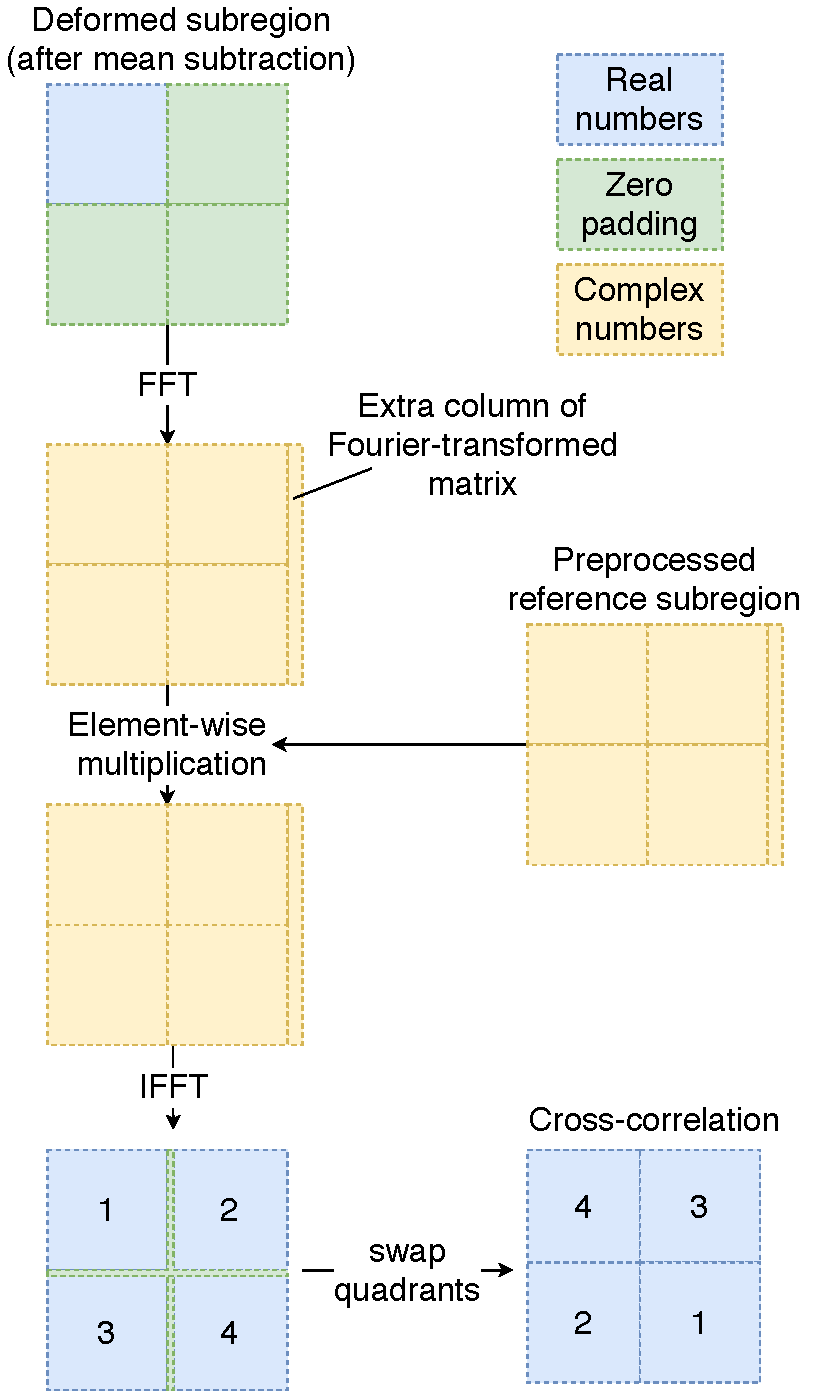
\includegraphics[width=0.7\textwidth]{img/fft-impl}
	\caption{The process of computing cross--correlation using the discrete Fourier transform.}
	\label{fft-impl}
\end{figure}

The last step to get the cross--correlation is to swap the quadrants of the result. The most straightforward solution is to start a kernel which does just that and thus finalizes the cross--correlation. Such kernel moves a considerable amount of data around and thus is relatively expensive. Instead, we can modify the rest of the implementation, so it accesses the data in corresponding way. In the next steps, we need to find the position of the maximal value in the cross--correlation and then process the neighborhood of the maximum. It can be easily modified to work with incomplete cross--correlation with swapped quadrants. The search of maximum stays the same and outputs the position of maximum, which then has to be interpreted correctly when fetching the neighborhoods to process them. This trick removes the overhead of running the extra kernel at the cost of more complicated, but only slightly more demanding data address calculation. Moreover, it works with much less amount of data, as the neighborhoods are only a small part of the cross--correlation.

\vspace{5px}

To sum up, we have described two ways to compute cross--correlation. The first one is based on the definition, the second one uses the Fourier transform which makes it possible to achieve better asymptotic time complexity. However for smaller input sizes, the definition--based approach is faster --- we measure that in chapter 3.


\section{Sum computation}
\label{sums}

Computation of sum is a textbook example of parallel reduction. In \cite{parallelReduction}, Justin Luitjens explains how to implement it on modern GPUs. Since it is very expensive to communicate between arbitrary threads during computation, the reduction is separated into three steps: first, each thread loads several values and computes their sum, then we reduce the data within each block individually and finally we synchronize single value for each block. The major difference for our case is that we compute a sum for each of several subregions, instead of reducing over the whole input data. The problem is that we cannot load values of two different subregions into one block. We solve this by assigning whole blocks to the subregions rather than just assigning threads to pixels.

Let $K$ be number of values that each thread loads, $B$ denote one block size and $P$ total number of pixels in one subregion, respectively. Then we use a group of $S_1~=~\ceil{\frac{P}{KB}}$ blocks for reduction of each subregion. If $P$ is not divisible by $KB$, then the last block in each group is not fully utilized, and processes only $K - 1$ values because there are no more pixels in the subregion.

\XX{For We measure the impact of the parameter in section ??. The problem is that half of the threads do (almost) nothing useful in the whole reduction: each of them only loads one value in the very beginning and immediately passes it to another thread (using shuffle instruction) which does the actual sum. So instead of loading only one value, each thread loads $N$ values and all the threads are utilized in the first part of the algorithm. It also means that we need $N$ times less blocks which may cause that for too high $N$, there will not be enough blocks to utilize the GPU.}

Once each thread loads its data, it is possible to reduce them fast within each block. We use warp--level shuffle instructions, which allows the threads in one warp to exchange data in registers. \Cref{warp_reduce} shows how it is possible to get sum of values in 8 threads. It can be expanded to size of warp, i.e. 32 threads. To reduce the whole block, we use the warp reduction in two steps:
\begin{enumerate}
	\item We perform the reduction within each warp and save the values into shared memory.
	\item One warp loads the values from the shared memory and reduces them using warp--level reduction again
\end{enumerate}
Maximum number of threads in one block is 1024 in CUDA and warp size is 32 so we get at most $1024/32 = 32$ values in the first step. That means one warp is enough to reduce them into one resulting value in the second step.

\begin{figure}
	\centering
	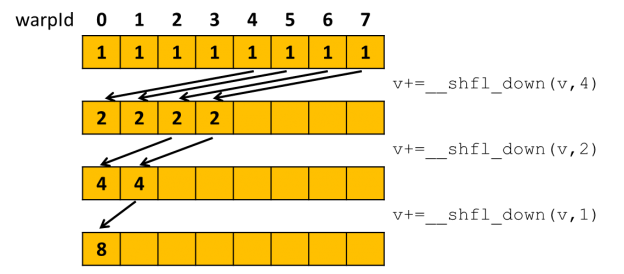
\includegraphics[width=0.7\textwidth]{img/warp_reduce}
	\caption{An example of warp--level reduction for 8 threads \cite{parallelReduction}. \emph{warpId} is a number of thread within its warp.}
	\label{warp_reduce}
\end{figure}

After the reduction within each block, we need to update the resulting values in global memory. If $S_1$ is equal to $1$, thus every subregion is processed by exactly one block, then there is no synchronization needed between the blocks. Otherwise, we can use \emph{atomic add}. The solution is feasible for us, since it is safe to assume that not many blocks access the same value. The worst case size of one subregion is $250 \times 250$ which is the total of 62500 pixels. \XX{ For $K = 1$ and $B = 1024$ (there is no reason not to use the maximal possible value --- no register or shared memory pressure), then 63 blocks compute the sum of one subregion.}. 


\section{Arg max computation}
The cross--correlated data are further processed to find the position of maximum for each subregion by using parallel reduction. The computation is very similar to the sums reduction explained in \cref{sums} we use warp--level shuffle instructions and shared memory to reduce the values loaded to each block. The difference compared to sum reduction is that we need to find the maximum and its position at the same time. So throughout the algorithm, we operate on the pair of value and its position. Every time we compare two values and choose the higher one, we propagate its position as well.

Otherwise the reduction within one block is analogous to the sum reduction. In each step we shuffle down the current value and its position (that means two shuffles per one step). Then we compare the received and current value and save the greater one with its position for the next step. We need five these steps to reduce one warp, then each warp saves its result to the shared memory. Finally, one warp reduces the items in the shared memory to get the result of one block reduction.

In the sums reduction kernel, we used built-in atomic add to update the global memory with the result of block reduction. No such function exists for arg max, since we need to atomically compare two values and then update the position as well. There are several ways how do the update without the atomic operation.

\begin{description}
	\item[Launch second kernel] The first kernel does no synchronization between the blocks and each block just writes its reduced result to its reserved place in global memory. Then, we start second kernel which reduces the results of the first one. In the second kernel, all the values from one subregion are reduced by one block, so there is no synchronization needed anymore. 
	\item[One block reduces one whole subregion] We increase the number of values that each thread loads before the reduction, so only one block is needed to find the maximum of each subregion. Therefore, no synchronization across blocks is needed. Depending on the number of subregions, there is a possibility that this approach does not spawn enough blocks to fully utilize the GPU.
	\item[Atomic compare and swap (float data only)] We can use the atomic compare and swap (CAS) instruction to update the global memory atomically. There are not many blocks that would compete over the same piece of memory, so it is a viable solution. However, it can only be done when we compute the cross--correlation in single precision floating point type, since modern GPUs only support atomic CAS for 8 bytes. A double precision number is 8 bytes long itself, and we need to update the pair of value and its position. 
\end{description}

The different approaches are compared in chapter 3.



\section{Subregions preprocessing}
Once we have described the most important parts of the algorithm, we explain how they are used together. In the following section, we outline the preprocessing that is needed before we can cross--correlate the subregions. It incorporates several steps:
\begin{enumerate}
	\item Load an image from disk
	\item Transfer the image from host memory to GPU memory
	\item Split the image into subregions
	\item Compute the sums of subregions
	\item Subtract the respective sums from subregions
\end{enumerate}




\section{Implementation overview}

\begin{figure}
	\centering
	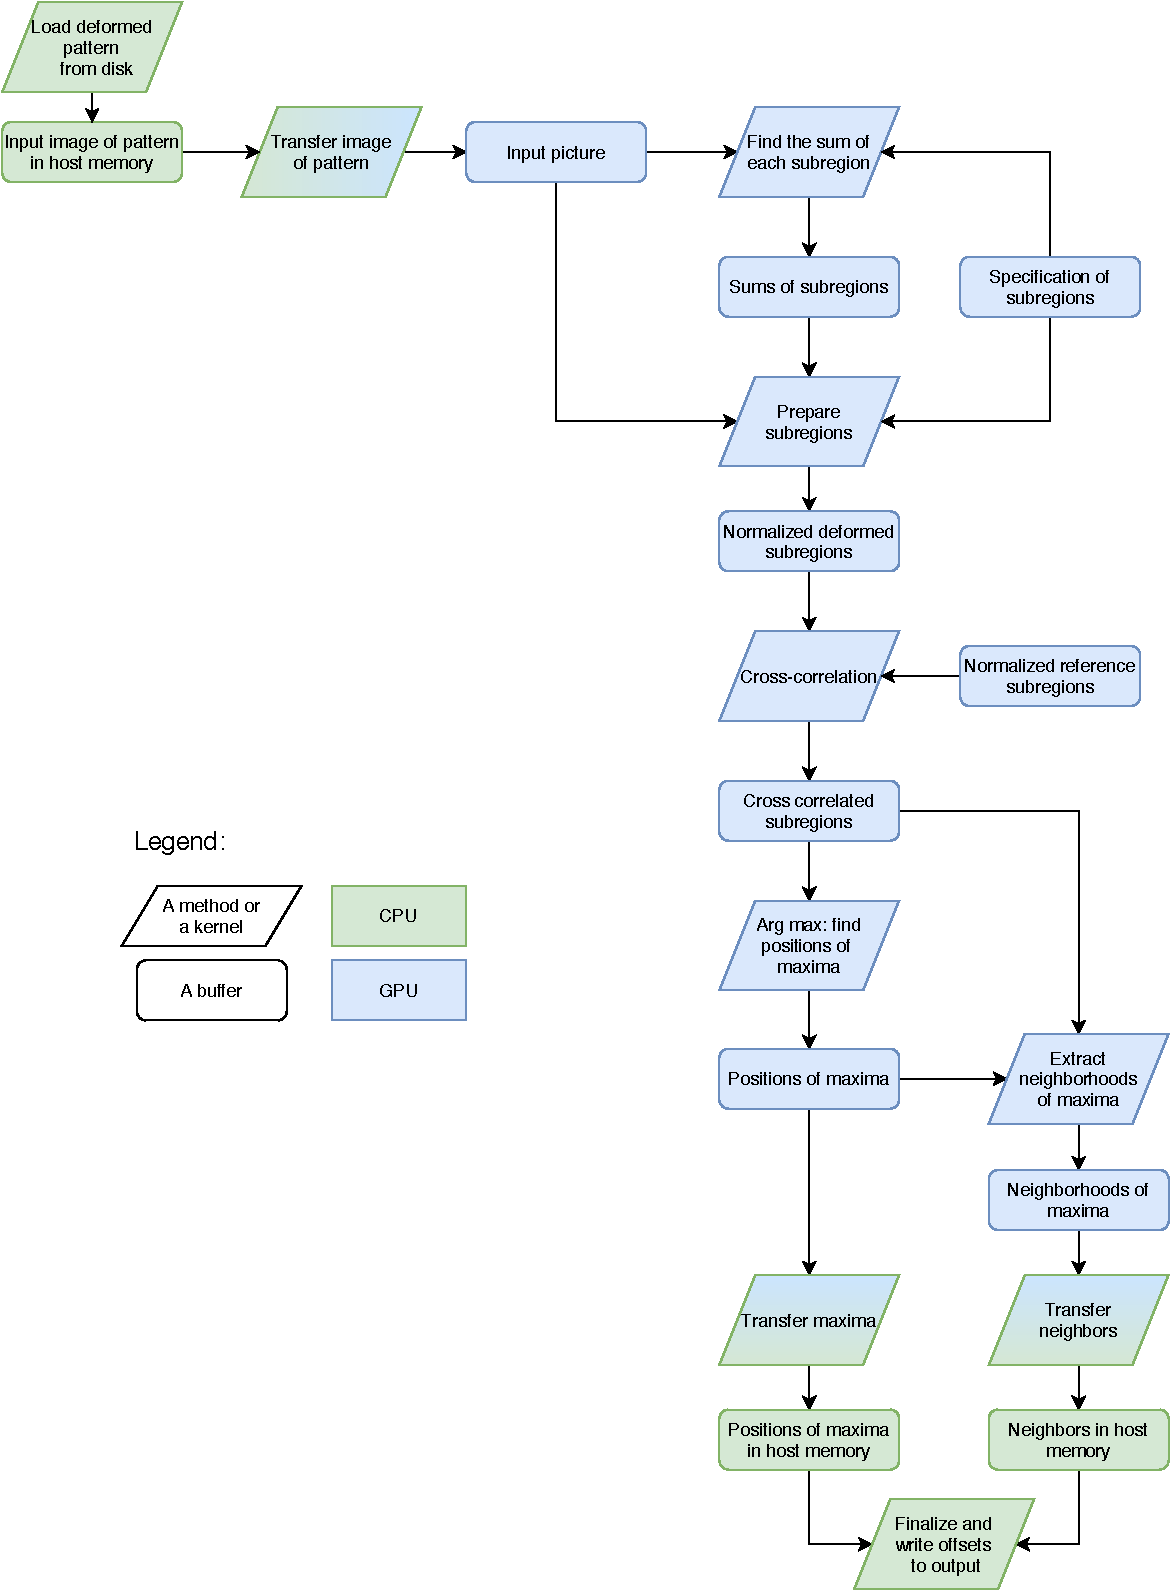
\includegraphics[width=\textwidth]{img/overview}
	\caption{Processing of one deformed pattern.}
	\label{overview}
\end{figure}

\Cref{overview} shows the data flow of the implementation and its decomposition into kernels. The processing starts with loading an image of a pattern from disk and its transfer to GPU. We transfer the whole pattern, as opposed to transferring only the subregions of interest.  Although we may end up copying data that the GPU never uses, this approach turned out to be better, because then we can utilize GPU when copying the subregions from the pattern. Moreover, we expect the regions to overlap in typical use case, so transferring the whole pattern copies less data.

The image is represented as an array of all the pixels in row--major order. Each pixel is an unsigned integer. 

Next, we need to prepare the data for cross--correlation --- copy the subregions from the image of deformed pattern and normalize them by subtracting the respective means. It is done in two kernels: \emph{sums} kernel and \emph{prepare} kernel. The sums kernel computes the sum of pixels of each subregion using parallel reduction. The prepare kernel extracts the subregions from the pattern, so that they are organized one after another in the output buffer: first, there all the pixels of the first subregion in row--major order, then all the pixels from the second and so on. Moreover, the kernel uses the sums from the first kernel to compute the mean for each region and subtracts it from each pixel of respective subregion.

The following part cross--correlates the normalized deformed subregions with reference ones. Since each deformed pattern is compared to the same reference, we pre-compute it (i.e., subtract the means from its subregions) and store it in a buffer on the GPU before loading the first deformed pattern.

Then, we analyze the result of the cross--correlation --- we find where is the maximum of each subregion using parallel reduction (\emph{arg max} kernel). The result is an array of coordinates of the maximum values (we are not interested in the values themselves). The next kernel then extracts a square shaped neighborhood of each maximum into one continuous buffer, so it can be transferred to the CPU memory together with the positions of the maxima.

The last part of the algorithm fits a continuous quadratic function to the neighborhood and then finds its maximum. We did not implement it for GPU, because it is not computationally demanding. It processes only a small neighborhood compared to the expected size of subregions. That also makes it cheap to transfer the maxima and neighborhoods from GPU to finish the computation on CPU and write the results to the output.

The decomposition into kernels is mostly determined by the need of global barriers. Both finding of sum and arg max use parallel reduction, which has to fully finish before any of its results are complete. The kernel that extracts the subregions from the pattern is necessary to simplify the cross--correlation and allow usage of third party libraries (see \cref{fft}, where the implementation of cross--correlation is explained).

To illustrate the data flow better and reason about it, \cref{params} summarizes parameters of the algorithm and \cref{buftypes} shows all buffers used on GPU with their sizes. The kernels that compute sums and normalize the subregions both work with $W_r \cdot H_r \cdot S$ items (i.e. all subregions). The cross--correlation has nearly four times as big output, which is then processed by the arg max kernel. After the maximum reduction, the buffers that are transferred to the CPU memory are quite small.

\begin{table}[]
	\begin{tabular}{@{}lll@{}}
		\toprule
		Buffer                          & Type         & Number of elements             \\ \midrule
		Input picture                   & uint16       & $W_p \cdot H_p$                \\
		Sums of subregions              & uint32       & $S$                            \\
		Positions of subregions         & uint32 pair  & $S$                            \\
		Normalized deformed subregions  & float/double & $W_r \cdot H_r \cdot S$        \\
		Normalized reference subregions & float/double & $W_r \cdot H_r \cdot S$        \\
		Cross--correlated subregions    & float/double & $(2W_r-1)\cdot(2H_r-1)\cdot S$ \\
		Positions of maxima             & uint32 pair  & $S$                            \\
		Neighborhoods of maxima         & float/double & $F^2 \cdot S $                 \\ \bottomrule
	\end{tabular}
	\caption{Summary of GPU buffers with their data types and size.}
	\label{buftypes}
\end{table}

The \cref{buftypes} also shows the data types stored in the buffers. The input image consists of unsigned 16 bit integers, so 4 byte unsigned integer is enough to hold the sums of its subregions of expected size. Once the means are subtracted, we use single or double floating point type --- when computing with 4 byte float, the implementation is substantially faster, however we are not sure whether it is precise enough, so we leave the choice as a parameter for our implementation.

\subsection{Task parallelization}

Since some parts of the algorithm are done on CPU and some on GPU (see color distinction in \cref{overview}), it is possible to parallelize them. There are 3 parts separated by data transfers between the main and the GPU memory: CPU first loads a pattern, GPU processes it, and then CPU does the finalization of results. It is desirable that we parallelize those tasks, so that GPU is fully utilized and never waits for the CPU.

\begin{figure}
	\centering
	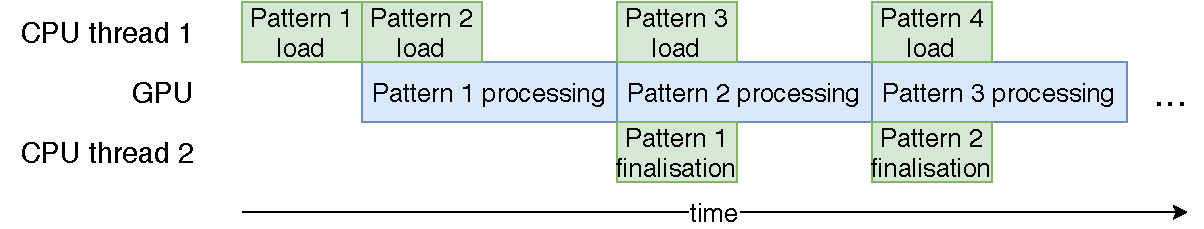
\includegraphics[width=\textwidth]{img/CPUGPUparal}
	\caption{Parallelization of GPU and CPU work.}
	\label{pipeline}
\end{figure}

\Cref{pipeline} shows how the work can be can be parallelized using a pipeline-like design. We use 2 worker CPU threads. While the GPU processes $i$-th pattern, one CPU thread already loads pattern $i+1$ and the second thread finalizes pattern $i-1$. The CPU work still takes much less time, so it is enough to start the load of pattern $i$ once processing of pattern $i-2$ finishes (and processing $i-1$ starts). That way, we do not need queues to pass work (like in the common pipeline pattern), we just need 2 buffers: one for writing the processed/prepared data and one for reading data to process. In the next iteration, we just swap the buffers.

We also partially take advantage of the fact that GPUs are able to run a kernel, copy data from and to memory at the same time. Actually, all transfers run in parallel with kernel execution. The host--device copy of input takes place right after the CPU loads the pattern from disk. Similarly, once the maxima and neighborhoods are prepared on the GPU, we start asynchronous transfer of the results and GPU starts computing the next pattern immediately. Unfortunately, this optimization does not affect performance much, since the copying between GPU and CPU memory takes only a marginal fraction of overall time.

In the following sections, we describe the implementation details of each individual kernel.


\section{Prepare kernel}
Once the sums are computed, we need to subtract them from each pixel of respective subregion. We use the \emph{prepare} kernel to do that and to copy the subregions from the pattern so they are stored continuously in one buffer. If some subregions are overlapping, we copy some of the data twice, but then we subtract different means from them in general, so the result does not have any duplicities.

The kernel is fairly straightforward, we assign one thread to each pixel in each subregion. The threads compute the position of their pixel in the pattern using the buffer with the positions of the subregions, then compute mean using the sums buffer, subtract it and finally write the value to the output buffer.




\section{Extract neighbors kernel}

Once we compute the position of cross--correlation maximum for each subregion, we need to transfer the maxima and their neighborhoods from GPU to main memory so that the CPU can finalize and output the offsets. The maxima are already ready to transfer as a result of the arg max kernel, but we need to start another kernel to copy the neighborhoods from the cross--correlation into its own buffer, so we do not have to transfer the whole cross--correlation.

Recall that $F$ denotes the size of the square neighborhood. Given a maximum $[x_m, y_m]$, its neighborhood are the points $\{x_m - \frac{F-1}{2}, \cdots, x_m, \cdots, x_m + \frac{F-1}{2}\} \times \{y_m - \frac{F-1}{2}, \cdots, y_m, \cdots, y_m + \frac{F-1}{2}\}$ of cross--correlation. $F$ is always an odd number, so that the maximum is in the middle of the neighborhood. So the output buffer has size $F^2 \cdot S$, because each neighborhood has $F \cdot F$ points and there are $S$ subregions.

In the kernel, we assign one thread to each point of the neighborhood. Each thread computes the address of its point and copies it from the cross--correlation buffer to the neighborhoods buffer.

This kernel works with very small amount of data compared to other kernels, since $F$ is expected to be less than 10. Therefore the running time of this kernel is marginal and does not offer much space for improving overall running time.

\section{Offsets finalization}

When we have the positions of maxima and their neighborhoods lined up in two buffers, we transfer them to the CPU memory, since the finalization of the offsets takes place on the CPU. We compute the locations of maxima of the neighborhoods with subpixel accuracy as explained in \cref{subpixel-peak}. With the precomputed least squares matrix, the estimation of the quadratic function coefficients is a matter of one matrix--vector multiplication. Then, we compute the location of maximum of the quadratic function using two simple formulas. That gives us the location of the maximum relative to each neighborhood. In the final step, we combine the location of neighborhoods transfered from the GPU with the relative subpixel location of maxima within the neighborhoods and write out the resulting offset.

\chapter{Benchmarks}

In this chapter, we measure the performance of our implementation. We quantify the impact of different input size and algorithm parameters. In the end, we compare our implementation with an original python implementation of the algorithm.

All the data was measured using an NVIDIA RTX 3080 graphics card with Intel i5 6600K processor. We used an M.2 SSD disk.

\todo{methodology? Each value presented in this chapter is a mean of several runs of the whole algorithm. Every time, we start the whole computation and measure runs of all kernels and take average from all the runs of kernels within one run of application. We repeat the process several times with the same parameters and take the average, then start over with different set of parameters.}

We measure only square subregions, because it removes unnecessary complexity from the benchmarks. In theory, whole algorithm works also for rectangle--shaped subregions, but since we analyze the direction in which the subregions are shifted, the square should have the same dimensions in each direction.

\section{Relative performance of individual parts}

\begin{figure}
	\centering
	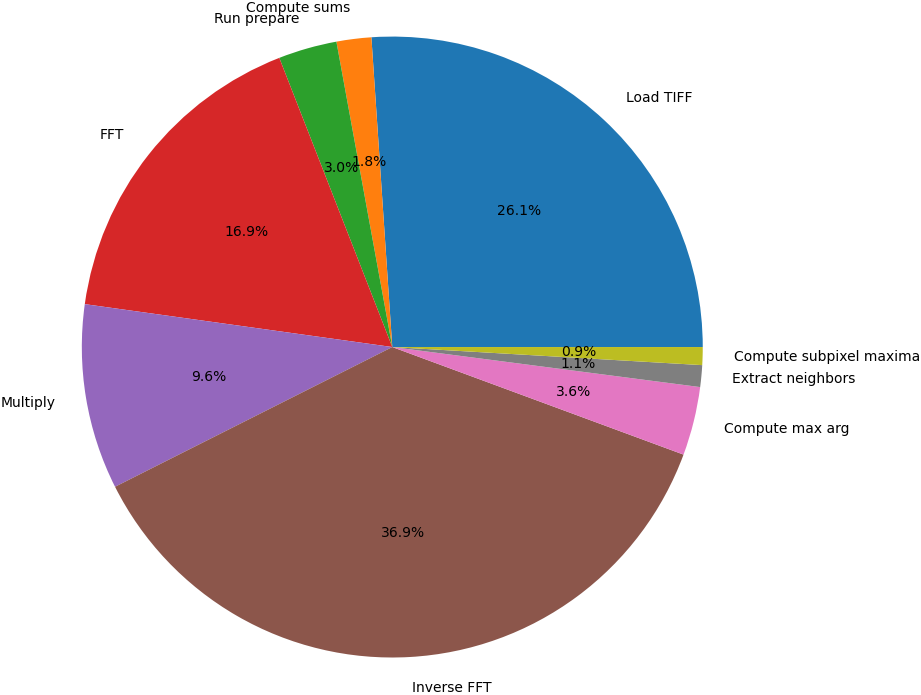
\includegraphics[width=0.7\textwidth]{img/eval/individual-parts}
	\caption{Relative performance of individual parts of the algorithm. The data was measured from a run of the algorithm with a configuration of 90 subregions with size $120 \times 120$. The size of the neigborhood was set to maximal value 9. }
	\label{individual-parts}
\end{figure}

We begin with an overview of all the kernels used in the implementation. \Cref{individual-parts} shows how much time the implementation spends in individual kernels. We can see, that the most demanding parts are loading of the TIFF and the cross--correlation, which is computed using the multiply kernel and the Fourier transforms.

The figure is mentioned here only to get general idea about the performance. It captures relative performance of the kernels for 90 subregions with size $120 \times 120$, which is roughly in the middle of the range of expected values. Different parts depend on different parameters, so for some other input size, the relative performance would look dissimilar. The load TIFF subroutine depends only on the size of the TIFF, while the rest of the algorithm depends on the number of subregion. So, for instance, it is possible to find a configuration that makes load TIFF the longest part. 

\section{Cross--correlation}
First, we measure the performance of cross--correlation when computed using Fourier transform. We show the dependence between running time and size and number of subregions. Since the cross--correlation is computed using three parts, we analyze them one by one.


\subsection{Fourier transforms}
\begin{figure}
	\centering
	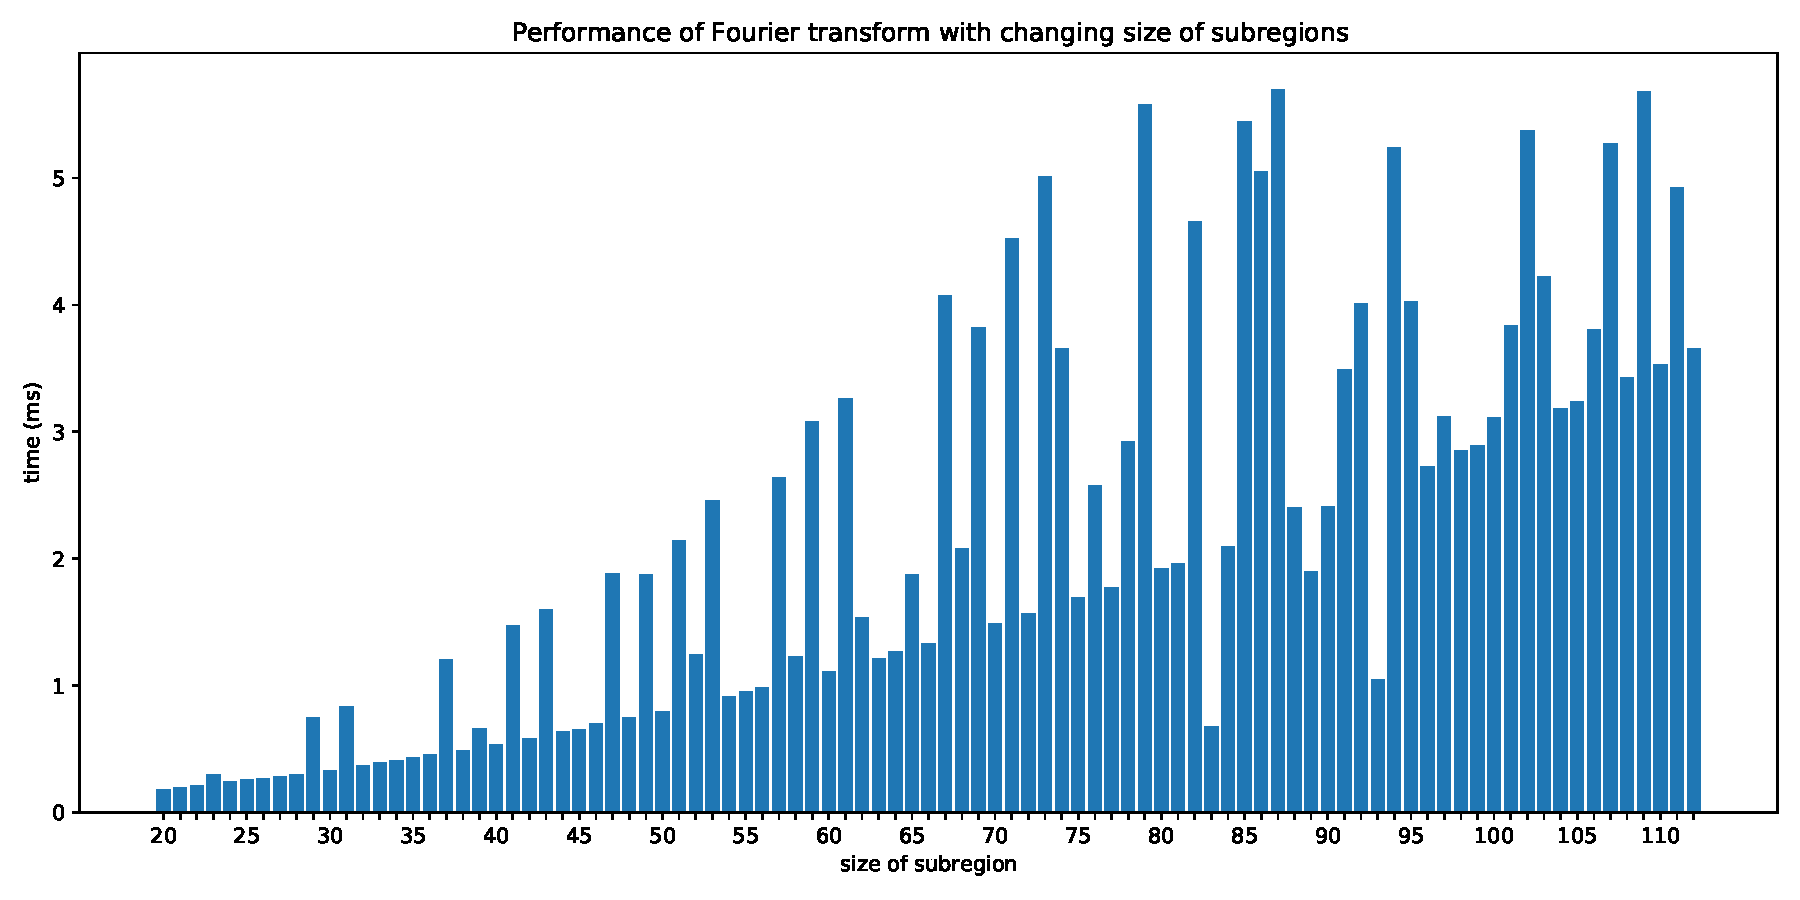
\includegraphics[width=\textwidth]{img/eval/Fourier-transform-size}
	\caption{Performance of Fourier transform with changing size of subregions. It was measured from a run of the algorithm with a configuration of 110 subregions. The size on the x axis denotes half of length of one side of subregion.}
	\label{Fourier-transform-size}
\end{figure}

In the \cref{Fourier-transform-size}, we can see how the forward Fourier transform executed by the cuFFT library depends on the size of subregions. We can see that the computation time increases with the size of the subregions, following the $\mathcal{O}(n \log n)$ time complexity of FFT, where $n$ is number of pixels. More precisely, the complexity is $\mathcal{O}(A^2 \log A)$, if $A$ denotes the length of one side of the square subregion.

However, there are quite a few outliers --- sizes, for which the function does not perform very well. That can be explained by the following sentence cited from the cuFFT documentation: ``Algorithms highly optimized for input sizes that can be written in the form $2^a3^b5^c7^d$''. It means that all sizes, whose factorization contains a prime greater than 7 perform poorly. Choosing a bigger size with nice factorization results in better performance.

We can also see, that sizes 83 and 93 perform surprisingly well. We have measured this fact consistently. The reason behind such behavior is probably specific for cuFFT implementation.

The dependence of inverse Fourier transform on size of subregions looks very similar to the \cref{Fourier-transform-size} for the same reasons.

\begin{figure}
	\begin{subfigure}{.5\textwidth}
		\centering
		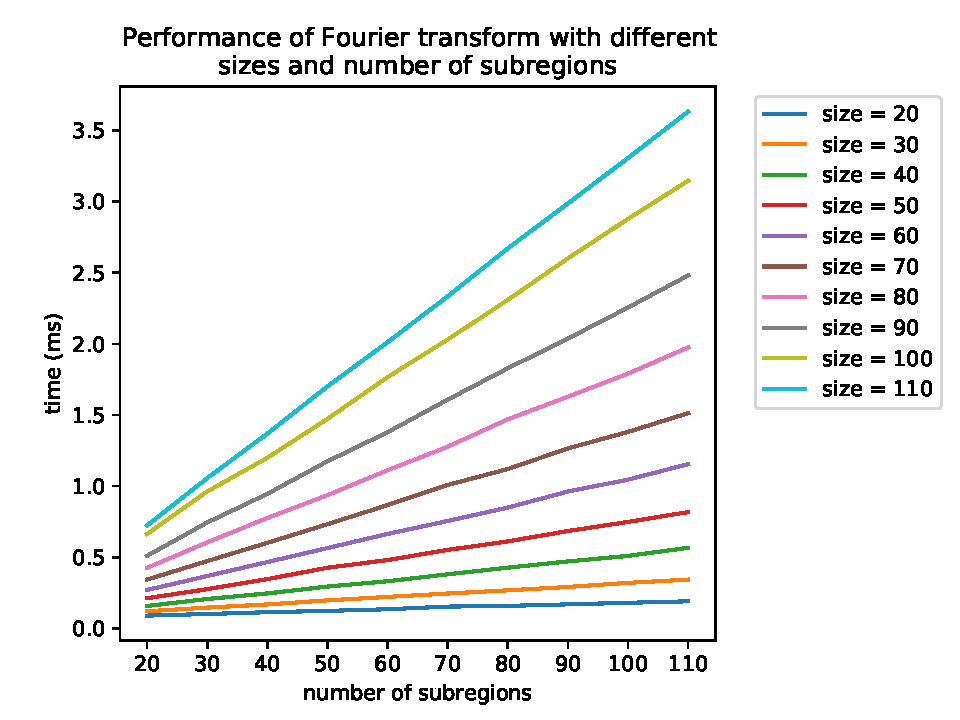
\includegraphics[width=\linewidth]{img/eval/fourier-transform-roi-count}
		\caption{}
		\label{fourier-transform-roi-count:basic}
	\end{subfigure}%
	\begin{subfigure}{.5\textwidth}
		\centering
		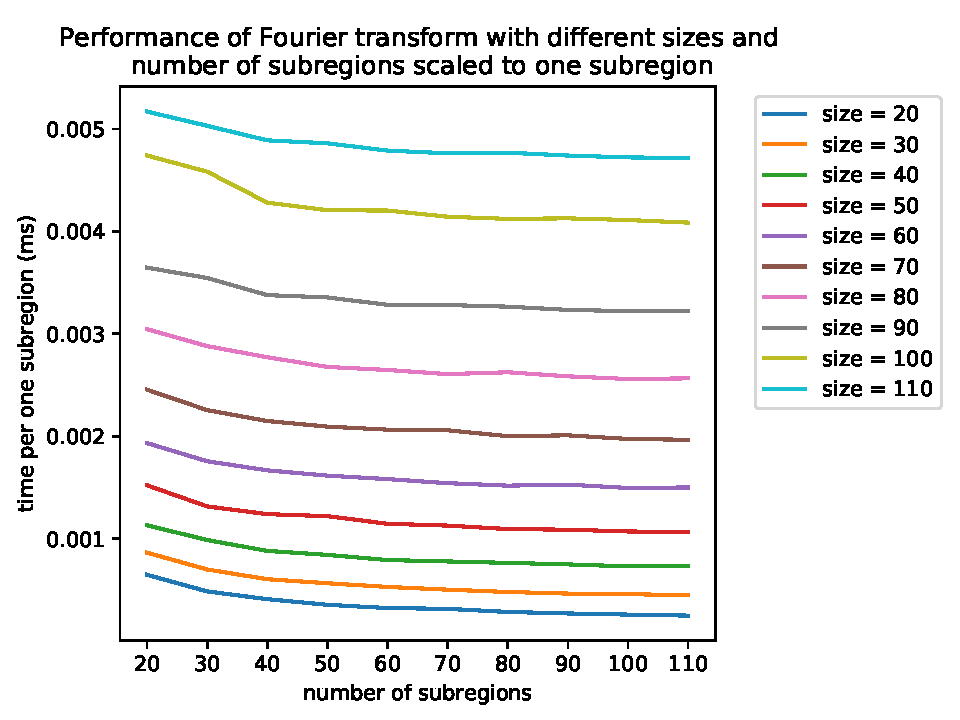
\includegraphics[width=\linewidth]{img/eval/fourier-transform-roi-count-scaled}
		\caption{}
		\label{fourier-transform-roi-count:scaled}
	\end{subfigure}
	\caption{Performance of Fourier transform with changing size and number of subregions. The size on the x axis denotes half of length of one side of subregion.}
	\label{fourier-transform-roi-count}
\end{figure}

\Cref{fourier-transform-roi-count} shows how the the Fourier transform performs with different sizes and number of subregions. \Cref {fourier-transform-roi-count:basic} shows absolute time it takes to compute the Fourier transform. As expected, the time scales roughly linearly with the number of subregions in each image.

\Cref {fourier-transform-roi-count:scaled} shows the same dependence, but the times are scaled with respect to number of subregions, so the y axis shows the average time needed to compute the Fourier transform of one subregion of respectable size. We can see that regardless of the size of subregions the library needs less time per subregion with increasing number of subregions. It is most likely caused by overhead of each CUDA kernel call --- with more subregions, the same overhead is spread over more of them, thus the computation of each subregion is cheaper. That is also the reason why we introduced the batch parameter --- to process more subregions in each run of kernel. We evaluate the impact of the batch parameter to the whole algorithm in \cref{batch-param}.

\subsection{The complex matrix multiplication}
\begin{figure}
	\begin{subfigure}{\textwidth}
		\centering
		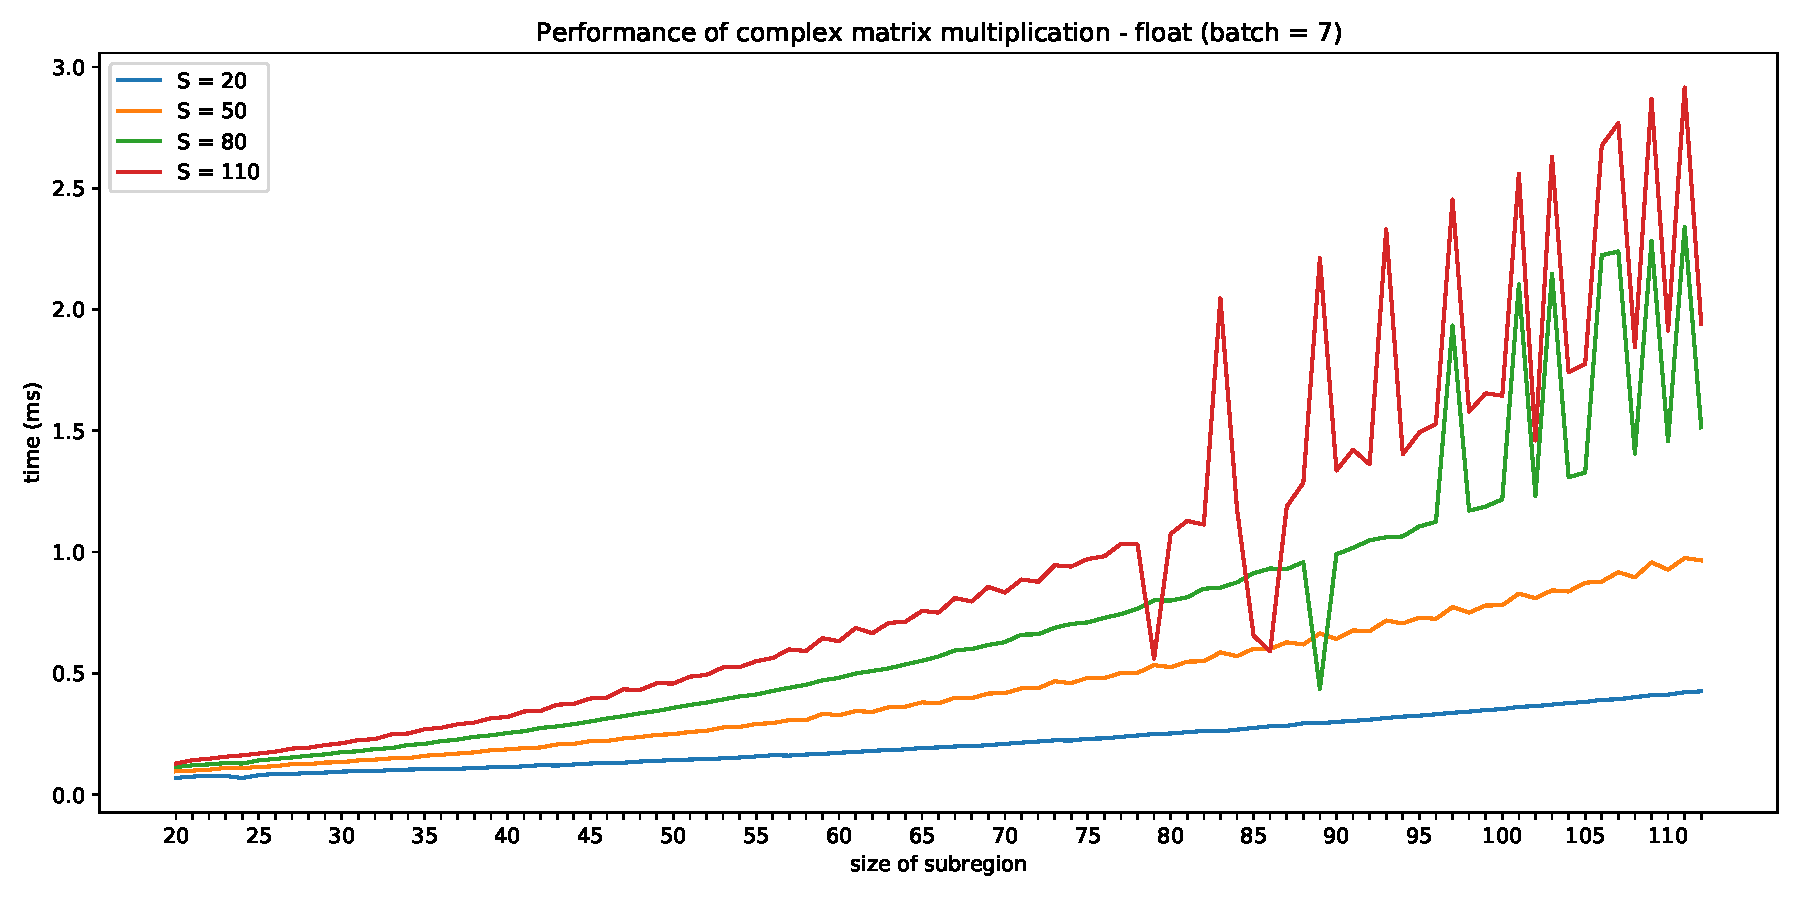
\includegraphics[width=\linewidth]{img/eval/multiply-plot-float}
		\caption{Single float precision}
		\label{multiply-plot:float}
	\end{subfigure}%

	\begin{subfigure}{\textwidth}
		\centering
		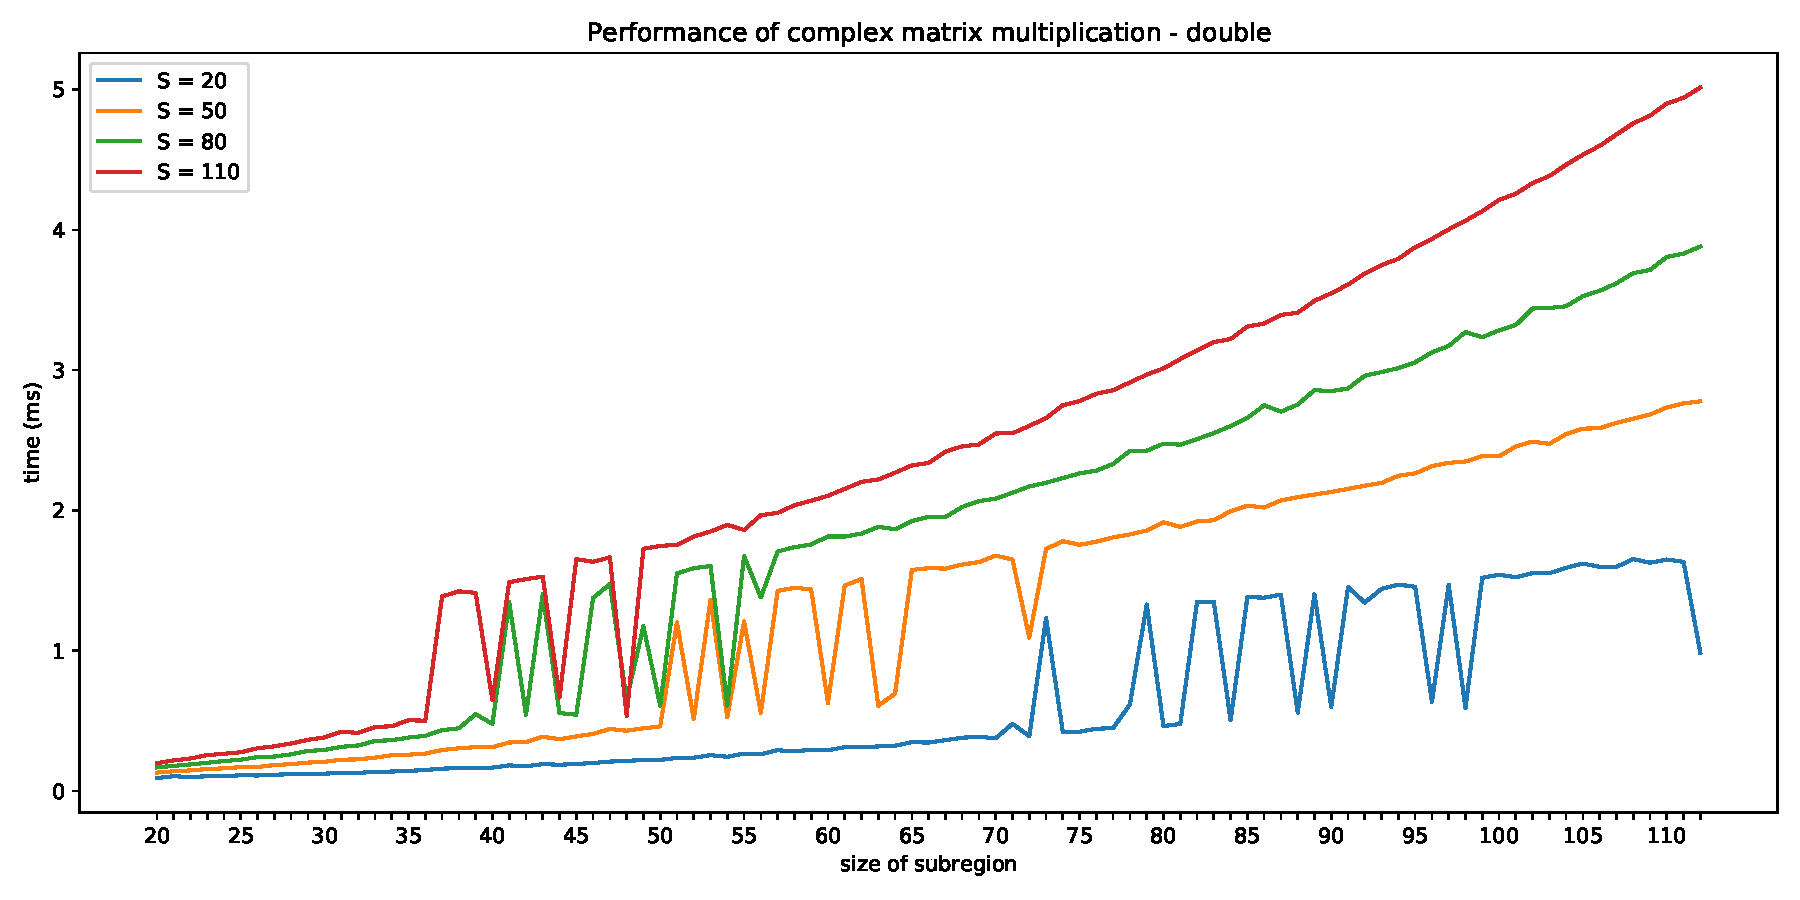
\includegraphics[width=\linewidth]{img/eval/multiply-plot-double}
		\caption{Double float precision}
		\label{multiply-plot:double}
	\end{subfigure}
	\caption{Performance of complex matrix multiplication with changing size and number of subregions. The size on the x axis denotes half of length of one side of subregion.}
	\label{multiply-plot}
\end{figure}

Another step in the cross--correlation computation is the multiplication of two complex matrices. In theory, the complexity of the multiplication is $\mathcal{O}(A^2S)$, where $A$ denotes the length of one side of the square subregion and $S$ denotes their amount. \Cref{multiply-plot} shows the measured time for different sizes and number of subregions. We can see the quadratic trend with respect to subregion size and linear with respect to their count.

However, in some cases, there seem to be a threshold over which the kernel performs worse. For float precision (\cref {multiply-plot:float}), the thresholds are higher than for double precision (\cref {multiply-plot:double}) and we do not see a consistent increase of the time for the measured sizes, only individual spikes. Unfortunately, we cannot reliably determine the relation between the threshold and algorithm parameters. It seems that the data exceed some kind of cache, but we observe worse performance for such big sizes that the processed subregions are already bigger than tens of megabytes. The plots look similar for different batch sizes too.

Moreover, we tried to measure the performance of the multiplication kernel individually and the observed worse performance was not present --- we measured clean quadratic dependency on size of subregions. That implies it is a result of some interference with the cuFFT forward Fourier transform. That would also explain the spikes, since cuFFT behaves differently for sizes with primes in their factorization. In any case, the performance difference is roughly 1ms, which is up to 10\% of total running time of whole offsets computation.

\subsection{FFT implementation versus definition--based implementation}

\begin{figure}
	\centering
	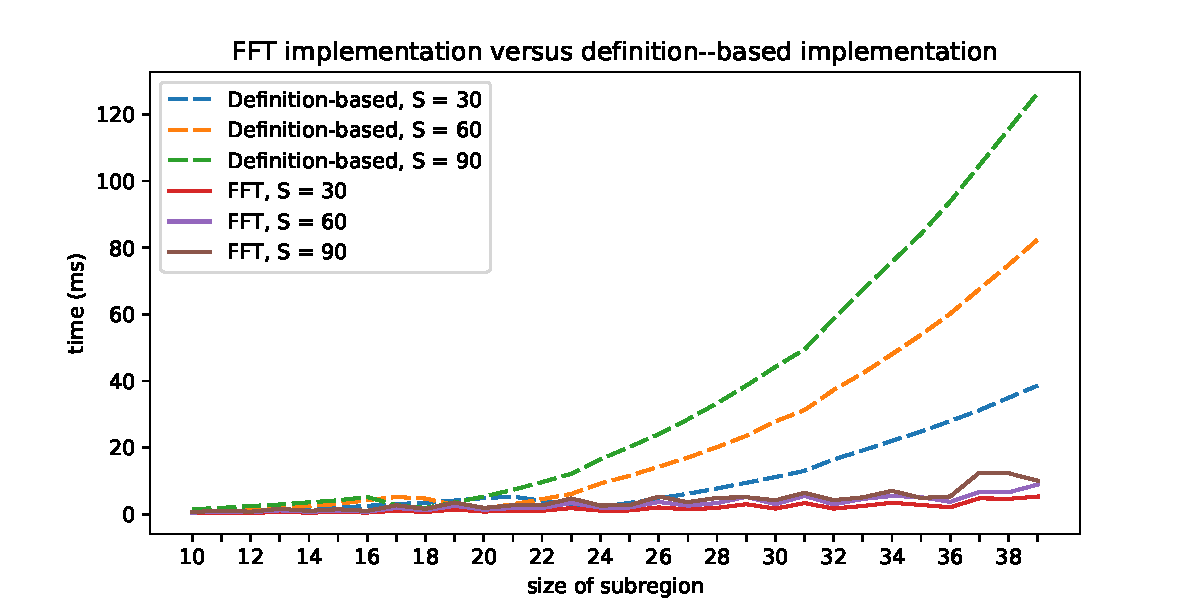
\includegraphics[width=0.8\textwidth]{img/eval/cross-compare}
	\caption{Comparison between the FFT and definition--based implementations of cross--correlation. The size on the x axis denotes half of length of one side of subregion.}
	\label{cross-compare}
\end{figure}

Recall, that we described two implementations of cross--correlation: first one based on the Fourier transform and second one based on the definition. \Cref{cross-compare} shows comparison between them --- for the FFT version, it shows the sum of average times of the Fourier transforms and complex multiplication. For the definition--based implementation, it shows the average run time of respective kernel. They are roughly the same for very small subregion sizes, but for sizes bigger than 25 the FFT implementation clearly wins. That is the minimal size of subregions that we consider useful for practical application. The conclusion is that the definition--based implementation is not useful for our application and it is always better to use the FFT implementation.


\section{Load TIFF}

\begin{figure}[h]
	\centering
	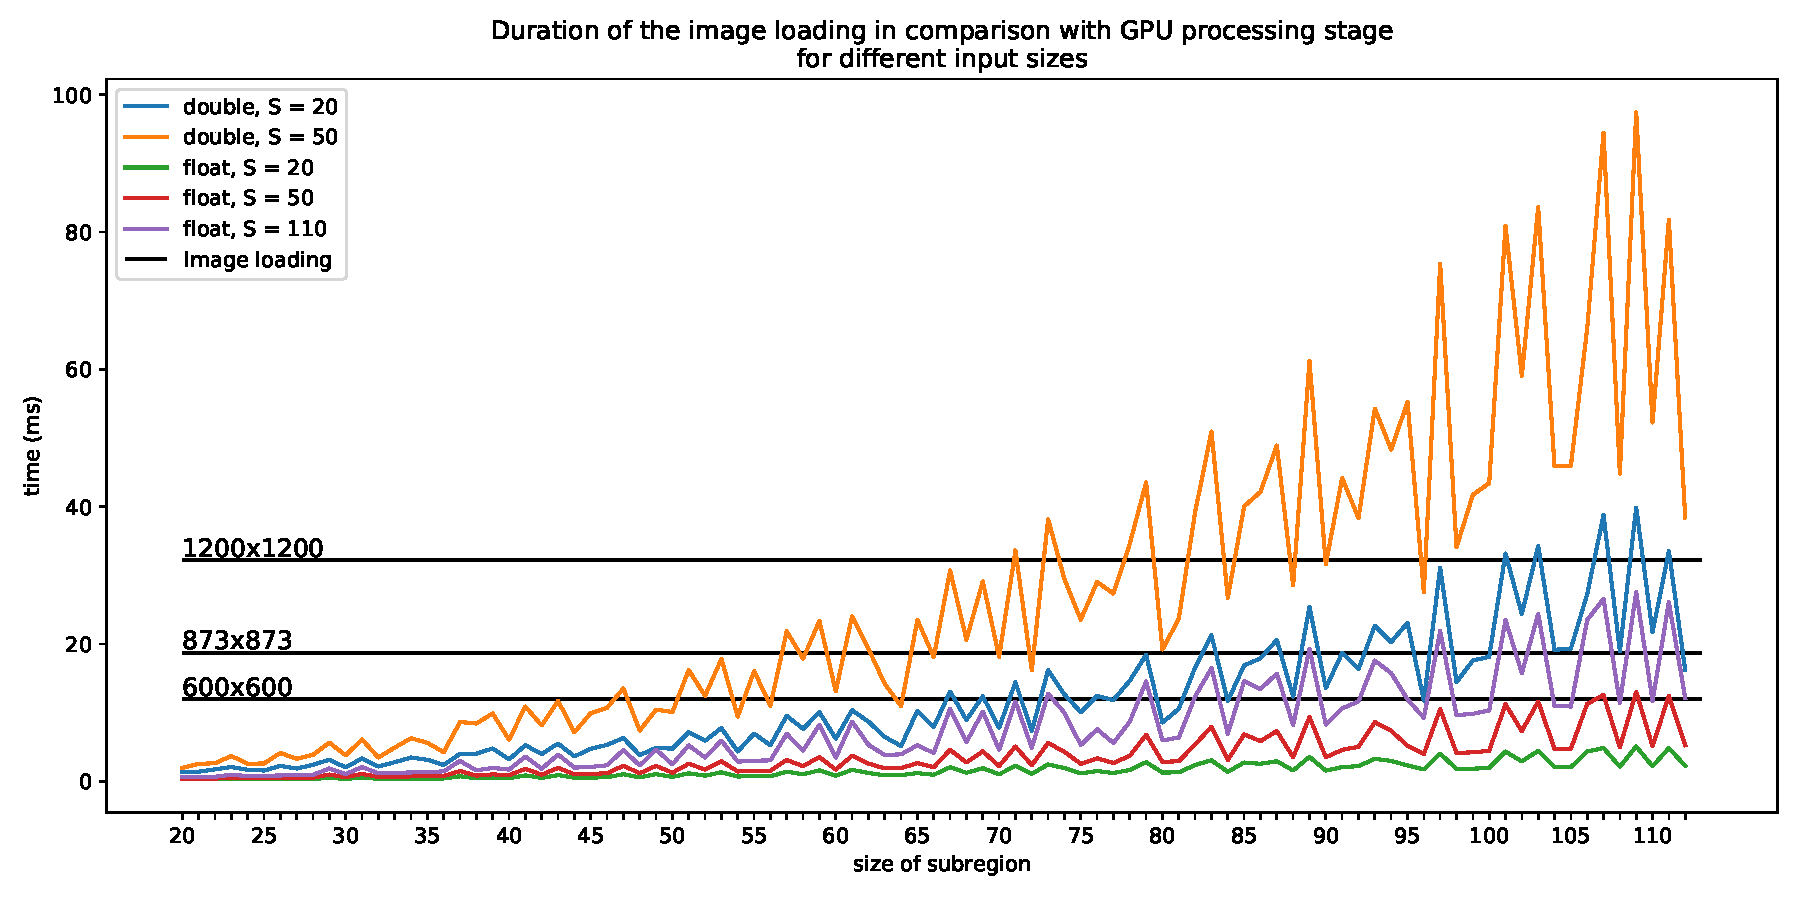
\includegraphics[width=0.8\textwidth]{img/eval/load-plot}
	\caption{}
	\label{load-wait}
\end{figure}

More workers

\section{Float versus double}


\section{Batch parameter}
\label{batch-param}


\section{Speedup compared to original python implementation}


\section{Memory consumption}


overall performance - compare with python

batch size for different subregion sizes and count

different subregion sizes and count

sum - compare N to size of one slice, to batch size, to number of slices - how?
\chapter*{Conclusion}
\addcontentsline{toc}{chapter}{Conclusion}

In this thesis we have described the processing of the Electron backscatter diffraction patterns (\cref{chap1}), including the cross--correlation and how is it computed using the Fourier transform(\cref{fft}). We have shown how is the cross--correlation subsequently processed to obtain estimation of the maximum position with subpixel precision (\cref{subpixel-peak}). The algorithm is summarized in pseudocode in \cref{algo-summary}.

Next, we have analyzed individual parts of the algorithm and described their CUDA implementations (\cref{chap1}). We have used the cuFFT library to compute the cross--correlation (\cref{fft-impl}) and used parallel reduction to implement kernels that find the sum of subregions (\cref{sums}) and the position of their maxima (\cref{arg-max}) --- the building stones of the algorithm. Then we described how to put them together as smoothly as possible and explained that the GPU processing can run in parallel with loading of input patterns {\cref{task-paralelization}}.

Finally, in \cref{chap3}, we have measured the performance of individual parts and compared to a reference python implementation, which runs on CPU and is even partly able utilize more cores (to implement the cross--correlation it uses an optimized multi--threaded Scipy function). We have achieved the speedup of 18 -- 40-times, for double floating precision, which yields the same results as the reference implementation. For single floating precision, we measured speedup of 18 to 270-times. We found out that especially the lower precision version (and the double version for small subregions) is bottlenecked by the throughput of contemporary consumer--grade M.2 SSDs (\cref{load-eval-lw}). Whether the higher performance of single float version is useful is up to physical interpretation of the error introduced by computation in lower precision.

Regardless of the precision, this thesis has the potential to considerably improve the EBSD processing. It improves the performance of EBSD data analysis closer to the speed of EBSD cameras, so now they are in the same order of magnitude at least for some parameters (it depends both on the settings of the camera as well as the analysis). Thus, all the data that the physicists are able to measure can be processed in similar time. Moreover, the improvement makes it possible to process bigger datasets in reasonable time.

\section*{Future work}

Although the implementation described in this thesis is useful and improves the EBSD analysis performance, it is only one part of the whole process. In the future, we need to make sure, that subsequent stages are able to efficiently process the subregion shifts produced by the program. It is possible that binary output of the implementation would be beneficial.

We can also see some possibilities to improve the performance of our solution itself. We have shown, that disk throughput, or even the CPU not being able to iterate through rather small chunks of TIFF fast enough, can limit the performance. The main goal of the thesis was the GPU implementation and we used libTIFF to load the patterns. Deeper analysis of the loading part or tighter adjustment for specific EBSD camera may result in better disk utilization

Should the GPU prove to be the bottleneck for chosen parameters, we also see further improvements there. One is to implement the algorithm for more GPUs. It should be pretty straightforward, since it is possible to add one worker to the GPU stage of the pipeline. And if the physicists evaluate, that single float precision is enough, it might be worth to implement the whole algorithm for half (16 bit) floating precision. 


%%% Bibliography
%%% Bibliography (literature used as a source)
%%%
%%% We employ bibTeX to construct the bibliography. It processes
%%% citations in the text (e.g., the \cite{...} macro) and looks up
%%% relevant entries in the bibliography.bib file.
%%%
%%% The \bibliographystyle command selects, which style will be used
%%% for references from the text. The argument in curly brackets is
%%% the name of the corresponding style file (*.bst). Both styles
%%% mentioned in this template are included in LaTeX distributions.

   %% Author (year)
% \bibliographystyle{unsrt}     %% [number]
%\bibliographystyle{alpha}

%\renewcommand{\bibname}{Bibliography}

%%% Generate the bibliography. Beware that if you cited no works,
%%% the empty list will be omitted completely.

%\bibliography{bibliography}

%%% If case you prefer to write the bibliography manually (without bibTeX),
%%% you can use the following. Please follow the ISO 690 standard and
%%% citation conventions of your field of research.

% \begin{thebibliography}{99}
%
% \bibitem{lamport94}
%   {\sc Lamport,} Leslie.
%   \emph{\LaTeX: A Document Preparation System}.
%   2nd edition.
%   Massachusetts: Addison Wesley, 1994.
%   ISBN 0-201-52983-1.
%
% \end{thebibliography}

%%% Figures used in the thesis (consider if this is needed)
\listoffigures

%%% Tables used in the thesis (consider if this is needed)
%%% In mathematical theses, it could be better to move the list of tables to the beginning of the thesis.
\listoftables

%%% Abbreviations used in the thesis, if any, including their explanation
%%% In mathematical theses, it could be better to move the list of abbreviations to the beginning of the thesis.
\chapwithtoc{List of Abbreviations}

%%% Attachments to the master thesis, if any. Each attachment must be
%%% referred to at least once from the text of the thesis. Attachments
%%% are numbered.
%%%
%%% The printed version should preferably contain attachments, which can be
%%% read (additional tables and charts, supplementary text, examples of
%%% program output, etc.). The electronic version is more suited for attachments
%%% which will likely be used in an electronic form rather than read (program
%%% source code, data files, interactive charts, etc.). Electronic attachments
%%% should be uploaded to SIS and optionally also included in the thesis on a~CD/DVD.
%%% Allowed file formats are specified in provision of the rector no. 72/2017.
\appendix
\chapter{Attachments}

\section{First Attachment}

\openright
\end{document}
